\documentclass[article,12pt,openany,oneside,a4paper,english,brazil]{abntex2}

% ---
% Pacotes fundamentais 
% ---
\usepackage{times}								% Usa a fonte Latin Modern
\usepackage{enumitem,amssymb}
\usepackage[T1]{fontenc}							% Selecao de codigos de fonte.
\usepackage[utf8]{inputenc}							% Codificacao do documento (conversão automática dos acentos)
\usepackage{indentfirst}							% Indenta o primeiro parágrafo de cada seção.
\usepackage{color}									% Controle das cores
\usepackage{graphicx}								% Inclusão de gráficos
\usepackage{microtype} 								% para melhorias de justificação
\usepackage{lipsum}									% para geração de dummy text
\usepackage[brazilian,hyperpageref]{backref}	 	% Paginas com as citações na bibl
\usepackage[alf]{abntex2cite}						% Citações padrão ABNT
\usepackage{tabularx}
\usepackage{multirow}
\usepackage{float}
\usepackage{tasks}

\hyphenation{en-si-no-a-pren-di-za-gem}

%\renewcommand{\familydefault}{\sfdefault}

\usepackage{fatec_capa}

% --- 
% CONFIGURAÇÕES DE PACOTES
% --- 

% ---
% Configurações do pacote backref
% Usado sem a opção hyperpageref de backref
\renewcommand{\backrefpagesname}{Citado na(s) página(s):~}
% Texto padrão antes do número das páginas
\renewcommand{\backref}{}
% Define os textos da citação
\renewcommand*{\backrefalt}[4]{
	\ifcase #1 %
		Nenhuma citação no texto.%
	\or
		Citado na página #2.%
	\else
		Citado #1 vezes nas páginas #2.%
	\fi}%

\newlist{todolist}{itemize}{2}
\setlist[todolist]{label=$\square$}
% ---

% ---
% Informações de dados para CAPA e FOLHA DE ROSTO
% ---

\titulo{Planejamento e desenvolvimento de um \textit{Serious Games} para educação básica}
\autor{Estudante: Fabrício Pinto Ferreira \\Orientador: Kleber de Oliveira Andrade}
\local{Americana}
\data{Agosto/2020 a Agosto/2021}
\instituicao{FACULDADE DE TECNOLOGIA DE AMERICANA
  \par TECNÓLOGO EM JOGOS DIGITAIS
  \par PROPOSTA DE PROJETO DE INICIAÇÃO CIENTÍFICA
  \par``CATEGORIA I: PESQUISA TECNOLOGICA''}
% ---

% ---
% Configurações de aparência do PDF final

% alterando o aspecto da cor azul
\definecolor{blue}{RGB}{41,5,195}

% informações do PDF
\makeatletter
\hypersetup{
     	%pagebackref=true,
		pdftitle={\@title}, 
		pdfauthor={\@author},
    	pdfsubject={\imprimirpreambulo},
	    pdfcreator={LaTeX with abnTeX2},
		pdfkeywords={abnt}{latex}{abntex}{abntex2}{projeto de pesquisa}, 
		colorlinks=true,       		% false: boxed links; true: colored links
    	linkcolor=blue,          	% color of internal links
    	citecolor=blue,        		% color of links to bibliography
    	filecolor=magenta,      		% color of file links
		urlcolor=blue,
		bookmarksdepth=4
}
\makeatother
% --- 

% --- 
% Espaçamentos entre linhas e parágrafos 
% --- 

% O tamanho do parágrafo é dado por:
\setlength{\parindent}{1.3cm}

% Controle do espaçamento entre um parágrafo e outro:
\setlength{\parskip}{0.2cm}  % tente também \onelineskip

% ---
% compila o indice
% ---
\makeindex
% ---

% ----
% Início do documento
% ----
\begin{document}

% Retira espaço extra obsoleto entre as frases.
\frenchspacing 

% ----------------------------------------------------------
% ELEMENTOS PRÉ-TEXTUAIS
% ----------------------------------------------------------
% \pretextual

% ---
% Capa
% ---
\imprimircapa
% ---

% ---
% inserir o sumario
% ---https://www.overleaf.com/project/5c923d00289f39238a59dc35
\pdfbookmark[0]{\contentsname}{toc}
\tableofcontents*
\newpage
% ---

\newpage
\setlength{\absparsep}{18pt} % ajusta o espaçamento dos parágrafos do resumo
\begin{resumo}

A utilização de tecnologias, como ferramenta acessória no processo ensino-aprendiza\-gem, está cada vez mais presente e diversificada no ambiente das escolas. Se por um lado, tais tecnologias auxiliam o professor nos processos de elaboração e condução das aulas mediante o uso de equipamentos de multimeios e a apresentação de conteúdos disponíveis em mídias digitais, por outro lado, tem-se que tais recursos tecnológicos podem representar um desafio estimulador para as crianças nessa fase de construção e desenvolvimento do conhecimento dentro do ambiente escolar. As brincadeiras e jogos estão presentes no mundo infantil como forma natural de prazer e aprendizado. Não obstante, as crianças precisam dos jogos como meio de equilíbrio entre ela e o mundo, além do mais os jogos trazem a ludicidade que é primordial ao seu desenvolvimento. As crianças são fortemente atraídas por brincadeiras e jogos, em específico aqueles disponíveis em meios eletrônicos e digitais, fato este que torna tais recursos uma possível ferramenta potencializadora dos resultados relacionados ao processo ensino-aprendizagem. Assim, o presente projeto visa ao desenvolvimento de um jogo digital que possa servir de ferramenta facilitadora no processo ensino-aprendizagem, trazendo em si elementos que estejam de acordo com os normativos educacionais, tais como a Base Nacional Comum Curricular e o Referencial Curricular Nacional para a Educação Infantil, bem como servir de módulo de integração com os sistemas de controle acadêmico existentes.

\textbf{Palavras-chaves}: jogos educativos; \textit{serious games}; unity; educação infantil; educação de qualidade.

\end{resumo}

%%%%%%%%%%%%%%%%%%%%%%%%%%%%%%%%%%%%%%%%%%%%%%%%%%%%%%%%%%%%%%%%%%%%%
%%% INTRODUÇÃO
%%%%%%%%%%%%%%%%%%%%%%%%%%%%%%%%%%%%%%%%%%%%%%%%%%%%%%%%%%%%%%%%%%%%%
\section{Introdução} \label{sc:intro}

O mundo está cada vez mais conectado e tecnológico, é comum cada vez mais as crianças estarem inseridas nesse contexto, utilizando de tablets, smartphones, computadores etc. como forma de entretenimento, passatempo e mesmo educação.

Com tais transformações em nossa sociedade, uma das principais instituições que a compõe 
está em constante evolução, a escola. Grande parte dessa evolução se deve ao grande avanço tecnológico ocorrido nas últimas décadas, além da enorme quantidade de informações as quais estamos sujeitos diariamente, impactando, direta e indiretamente, em todos as etapas e fases da educação, bem como nos aspectos sociais e emocionais dos alunos.

O presente projeto, tem como tema precípuo a educação de crianças inseridas na etapa da educação infantil e no ensino fundamental I, utilizando de um jogo virtual educativo como ferramenta para tal, tendo como base para seu desenvolvimento documentos norteadores oficiais, como por exemplo a Base Nacional Comum Curricular (BNCC\footnote{\citeonline{Base2017}}), as Diretrizes Curriculares Nacionais da Educação Infantil (DCNEI\footnote{\citeonline{Diretrizes2013}}), o Referencial Curricular Nacional para a Educação Infantil (RCNEI\footnote{\citeonline{Referencial1998}}) etc.

É evidente a ausência ou a pouca oferta de soluções de tecnologia, principalmente em forma de jogos virtuais educativos, que sigam rigidamente a BNCC, que sejam eficazes, eficientes e seguras e que estejam disponíveis e acessíveis nas instituições educacionais para atuarem como coadjuvantes no processo de ensino-aprendizagem na etapa da educação infantil e no ensino fundamental I.

Além de que, é comum encontrarmos jogos, ditos infantis, que atraem as crianças e que até podem auxiliá-las na identificação de sons e cores, por exemplo, mas perdem a característica de jogos educativos e se tornam tão somente jogos de entretenimento ou casuais por não seguirem padrões normativos curriculares condizentes com nosso atual sistema de ensino, tais como a própria BNCC, as DCNEI ou o RCNEI.

Apesar desses entraves, os jogos virtuais educativos proporcionam diversão e apresentam benefícios a vida da criança, como por exemplo o desenvolvimento da coordenação motora, principalmente da coordenação motora fina, devido a manipulação delicada de controles, mouse e \textit{joysticks}, exigindo, em sua grande maioria, a combinação entre movimentos de olho e mão para que a criança execute a atividade.

O estímulo do raciocínio é outra vantagem de sua utilização, por meio de atividades que exigem o controle de personagens o jogador precisa usar da lógica e do raciocínio para executá-las, servindo de estímulo para o desenvolvimento de funções cognitivas, tais como a atenção e a memória. Ademais o grande desenvolvimento da criatividade com atividades lúdicas, como colorir, pintar, desenhar etc.

Atrelado a estes benefícios está também uma maior aproximação dos professores e pais ao mundo da criança, através de atividades coletivas que estimulam a interação entre os mesmos, criando espaços de socialização em sala de aula e fora dela.

%%%%%%%%%%%%%%%%%%%%%%%%%%%%%%%%%%%%%%%%%%%%%%%%%%%%%%%%%%%%%%%%%%%%%
%%% OBJETIVO GERAL
%%%%%%%%%%%%%%%%%%%%%%%%%%%%%%%%%%%%%%%%%%%%%%%%%%%%%%%%%%%%%%%%%%%%%
\section{Objetivo geral do projeto}
\label{sc:objetivo}

O  presente  trabalho  tem  como principais objetivos:
\begin{itemize}
    \item Desenvolvimento de um jogo digital sócio-educativo infantil, multiplataforma e multijogador, baseado nos campos de experiência voltados para a educação infantil contidos na BNCC, alinhado com os objetos de conhecimento que compõem o âmbito de referência “Conhecimento de Mundo” do RCNEI e com os princípios básicos das DCNEI;

    \item Disponibilização do jogo digital para utilização em instituições da rede pública de educação infantil e ensino fundamental I - fase inicial, através de convênios e parcerias;
    
    \item Treinamento para o corpo técnico-docente que lida diretamente com as crianças no ambiente escolar do público-alvo principal;
    
    \item Acompanhamento da evolução e validação da utilização e dos resultados junto ao público-alvo.
\end{itemize}

%%%%%%%%%%%%%%%%%%%%%%%%%%%%%%%%%%%%%%%%%%%%%%%%%%%%%%%%%%%%%%%%%%%%%
%%% OBJETIVOS ESPECÍFICOS
%%%%%%%%%%%%%%%%%%%%%%%%%%%%%%%%%%%%%%%%%%%%%%%%%%%%%%%%%%%%%%%%%%%%%
\section{Objetivos específicos}
\label{sc:obj_esp}

\begin{itemize}
    \item Desenvolver uma arquitetura de software que dê suporte a um \textit{framework} de jogo digital acadêmico multijogador e multiplataforma que apresentem as seguintes qualidades: Interoperabilidade, Segurança de acesso, Conformidade, Acurácia, Adequação, Usabilidade, Eficiência, Manutenibilidade e Portabilidade;
    \item Desenvolver um agente inteligente aplicado a fim de balancear os níveis de dificuldade dos obstáculos do jogo;
    \item Desenvolver um \textit{framework} conceitual genérico aplicável ao desenvolvimento de jogos virtuais socioeducativos aderente aos normativos da educação infantil e suas mutabilidades;
    \item Investigar os possíveis dispositivos de interação entre o jogo e o jogador, aplicáveis aos jogos virtuais socioeducativos voltados para o público infantil;
    \item Desenvolver multimeios acessórios, tais como: cartilhas, livretos, manuais, cursos, videoaulas, etc;
    \item Promover parcerias com instituições educacionais de ensino médio-técnico em informática para a disseminação das tecnologias e metodologias de desenvolvimento de jogos virtuais.
\end{itemize}

%%%%%%%%%%%%%%%%%%%%%%%%%%%%%%%%%%%%%%%%%%%%%%%%%%%%%%%%%%%%%%%%%%%%%
%%% JUSTIFICATIVA
%%%%%%%%%%%%%%%%%%%%%%%%%%%%%%%%%%%%%%%%%%%%%%%%%%%%%%%%%%%%%%%%%%%%%
\section{Justificativa}
\label{sc:just}

O mundo está cada vez mais conectado e as crianças estão mais que acostumadas com computadores, tablets e smartphones. 

Isso faz com que os jogos virtuais ganhem cada vez mais força e presença no dia a dia das crianças. Então, utilizar metodologias associadas à esta tecnologia para educar em sala de aula é uma maneira de aproximar os professores dos pequenos aprendizes e criar um ambiente moderno de aprendizado.

Os jogos virtuais socioeducativos já são alvos de estudos e discussões no ambiente educacional e passaram a ser usados por muitas escolas para fortalecer o processo de aprendizagem.
Muitas ferramentas facilitam o ensino de formas geométricas, das cores, do alfabeto, dos números, e de línguas estrangeiras, por exemplo, e ainda estimulam a função cognitiva do cérebro das crianças.

As escolas de educação infantil precisam se adaptar o quanto antes a esse contexto de ensino, unindo o processo ensino-aprendizagem e a utilização das tecnologias de jogos virtuais socioeducativos, para maximizar o interesse dos alunos e aprimorar os resultados do processo.

%% Exemplo de citação na linha
Para \citeonline{Schmidt2017}, quando os jogos digitais são usados de forma educativa, ou seja, com objetivos definidos para se alcançar um resultado significativo, abre-se possibilidades de aprendizagem como o desenvolvimento de diversas habilidades de cada sujeito, facilitando o convívio social, o desenvolvimento da motricidade, coordenação, raciocínio lógico e, ainda, os jogos são utilizados no desenvolvimento da atenção, concentração, autonomia, onde a criança vai gradativamente aprendendo a formar os seus próprios conceitos.

%% Exemplo de apud
%%Segundo \apudonline{Schmidt2017}{Schmidt2017}, os

Segundo \apudonline{Tarouco}{Schmidt2017}, os jogos educacionais se baseiam numa abordagem autodirigida, isto é, aquele em que o sujeito aprende por si só, através da descoberta de relações e interações com o software. Neste cenário, o professor tem o papel de moderador, mediador do processo, dando orientações e selecionando softwares adequados e condizentes com a sua prática pedagógica.

Ainda para \citeonline{Schmidt2017}, desse modo, a criança vai aprendendo por meio da descoberta da interação com o software, mas o professor passa a assumir o papel de mediador, no qual orientará o processo e auxiliará  nas dúvidas. Por isso, é importante que o professor conheça como manusear as tecnologias, para que assim ele possa auxiliar as crianças quando as dúvidas surgirem.

Nesse sentido, o professor na educação infantil, ao trabalhar com jogos educativos digitais, atua como um mediador que estabelece entre a criança e a ferramenta um aprendizado progressivo com a interação e o entretenimento fazendo com que a criança amplie seus conhecimentos.
Entre os benefícios da utilização dos jogos virtuais na educação infantil podem ser destacados:

\begin{enumerate}
  \item \textbf{Desenvolvimento da coordenação motora:}  Os jogos virtuais socioeducativos tanto proporcionam diversão para as crianças quanto exercícios para o corpo, dependendo das tecnologias utilizadas, e a mente. Em sua grande maioria, os jogos virtuais auxiliam no aprimoramento da coordenação motora fina, pois exigem a manipulação de peças e bonecos de forma delicada. Eles também exigem a combinação entre os movimentos do olho e da mão, para que a criança possa executar a atividade.
  
  \item \textbf{Estímulo ao raciocínio:} Incentivam as crianças a controlarem personagens e executarem ações que exigem lógica e raciocínio. Por isso, esses jogos, também, ajudam a melhorar a atenção e a memória das crianças e passam a servir de estímulo para o desenvolvimento de funções cognitivas.
  
  \item \textbf{Criatividade:} Estimulam a criatividade dos alunos desde cedo, com atividades tais como montar, colorir, cuidar do meio ambiente, praticar cidadania, entre outras.
  
   \item \textbf{Maior interação com professores, pais e demais colegas:} Servem como meio de aproximar ainda mais professores e pais do mundo da criança através de atividades coletivas estimulando, dessa forma, a interação com outras pessoas. O que facilita o convívio social e cria espaços para novas interações no ambiente da sala de aula.
  
\end{enumerate}

%%%%%%%%%%%%%%%%%%%%%%%%%%%%%%%%%%%%%%%%%%%%%%%%%%%%%%%%%%%%%%%%%%%%%
%%% REFERÊNCIAL TEÓRICO
%%%%%%%%%%%%%%%%%%%%%%%%%%%%%%%%%%%%%%%%%%%%%%%%%%%%%%%%%%%%%%%%%%%%%
\section{Referencial teórico}
\label{sc:ref}

De acordo com \apudonline{Takahashi}{Padilha2013}, a nossa compreensão de tempo, espaço e conhecimento foi afetada com a revolução da quantidade de informações, atingindo e modificando, de forma permanente, o funcionamento de diversas áreas, tais como educação, economia, lazer e cultura.

Em relação aos impactos psicológicos dos jogos eletrônicos na vida das crianças, tanto \apudonline{Lepikson}{Cotonhoto2016}, quanto  \apudonline{Ramos}{Cotonhoto2016} e \apudonline{Cairoli}{Cotonhoto2016} concluíram que os jogos influenciam no desenvolvimento cognitivo, social e emocional das crianças. Cognitivamente, a prática de jogos eletrônicos exige que as crianças sejam mais atentas, concentradas, façam planejamentos, avaliem e tomem decisões; na questão social, \apudonline{Lepikson}{Cotonhoto2016} e \apudonline{Ramos}{Cotonhoto2016} apontam ainda que as crianças tendem a jogar em pares ou em grupos, compartilhando informações, traçando estratégias, torcendo e incentivando o parceiro.

\apudonline{Ramos}{Cotonhoto2016} também aponta dados sobre a relação entre os jogos eletrônicos e a formação do juízo moral e transmissão das regras e valores sociais durante o desenvolvimento infantil. A autora questiona a função dos jogos eletrônicos na construção da moral, das regras e valores sociais na infância, preocupação essa que vai além da aprendizagem formal, do contexto escolar e envolve a participação da família e de profissionais ligados à área da psicologia do desenvolvimento.

Para \apudonline{Cairoli}{Cotonhoto2016}, ao investigar o brincar na contemporaneidade, também recorreu à psicologia para discutir a respeito da influência dos meios eletrônicos na produção de subjetividade das crianças. A partir de uma referência psicanalítica, a autora procurou evidências na literatura de que o brincar contemporâneo influência na constituição da subjetividade da criança, ou seja, é parte importante no desenvolvimento humano.

Assim, \citeonline{Cotonhoto2016} concluíram que as pesquisas sobre a prática de jogos eletrônicos na infância trouxeram, predominantemente, uma concepção implícita de jogo, e em especial o jogo eletrônico, como algo pedagógico e educativo. A área da educação domina as pesquisas sobre o tema, demonstrando não somente interesse e preocupação com esse fenômeno, mas determinando que essa prática deve estar sob a responsabilidade e determinação da pedagogia. A ausência de mais investigações na área da psicologia sugere um desinteresse ou desconhecimento dos profissionais e estudiosos em entender e analisar a prática do jogo eletrônico como um aspecto relevante do desenvolvimento infantil, dadas as transformações sociais, culturais e tecnológicas que vivemos.

Para \citeonline{Schmidt2017}, o uso da informática vem obtendo cada vez mais espaço e importância no cenário educacional, pois algumas ferramentas têm proporcionado significativas mudanças no processo de ensino aprendizagem de alunos. Assim, a maioria das tecnologias utilizadas na escola tornaram-se instrumentos aliados dos professores para facilitar a aprendizagem dos estudantes. Segundo \apudonline{Lopes}{Schmidt2017} houve época que era necessário justificar a introdução da informática na escola. Hoje já existe consenso quanto a sua importância. Entretanto, o que vem sendo questionado é a forma como essa introdução vem ocorrendo.

Ainda, segundo \citeonline{Schmidt2017}, as instituições de educação infantil precisam proporcionar ambientes de experiências únicas, nos quais as crianças possam criar e recriar sua maneira de agir e expressar. Além disso, deve-se oferecer situações pedagógicas intencionais que favoreçam o processo ensino-aprendizagem. E, uma dessas situações pode ocorrer por meio dos jogos educativos digitais, uma vez que os mesmos são desenvolvidos para entreter os alunos e possibilitar uma aprendizagem de conhecimentos, conteúdos e habilidades. Assim, nas escolas, os jogos digitais devem ser preparados como um recurso didático que agregue valores e benefícios para as práticas de ensino-aprendizagem, pois, conforme \apudonline{Tielllet}{Schmidt2017}, “um jogo bem projetado envolve interação, mantendo o interesse do aluno, enquanto desenvolve habilidades, socializa-se e auxiliando na construção do conhecimento e do raciocínio).

Para \citeonline{An2013} Os softwares educacionais, para estarem apropriados para o seu uso no processo de aprendizagem, devem seguir determinados critérios e serem avaliados quanto aos mesmos. Para autores com enfoque mais técnico, ligados à Ciência da Computação, as etapas que devem ser consideradas para o desenvolvimento do software educativo podem ser assim enumeradas: seleção do conteúdo; verificação dos conhecimentos prévios que se precisa; definição dos conceitos sobre a estrutura do conteúdo; elaboração do diagrama de fluxo; construção das telas e implementação das mesmas (diagrama de fluxo, documentação, layout e associação entre as telas); elaboração da documentação do software; uso, verificação e manutenção do software.

Ainda, segundo o trabalho de \citeonline{An2013}, além dessas, os jogos educativos também devem considerar os critérios que são baseados em teorias construtivistas e interacionistas. Dessa forma os desenvolvedores deveriam: sugerir ambientes que possibilitem o aprendizado sob múltiplas perspectivas; sugerir contextos compatíveis com o conhecimento além da sala de aula; possibilitar a interpretação significativa e reflexiva; estimular o pensamento crítico; fomentar a comunicação, de modo que haja troca de ideias e análise de diferentes alternativas e prover apoio ao aluno, ao contexto da aprendizagem e ao processo.

O software educativo precisa apresentar como um dos requisitos principais a usabilidade, além de produzir algum conhecimento. Deve seguir ainda outros critérios de características de qualidade, compatibilidade e tolerância a erros. Também devem apresentar um \textit{feedback} ao usuário que facilite o aprendizado, como pistas da resposta correta, levando a uma reflexão sobre seu erro, para que não seja apenas um jogo de tentativa e erro, o que não traria contribuição para o processo de aprendizado da criança. Sendo assim, além dos requisitos de qualidade comuns a outros programas computacionais, os jogos educativos precisam ter atributos pedagógicos, voltados para o aprendizado efetivo do seu público-alvo, no caso as crianças em processo de alfabetização.

%%%%%%%%%%%%%%%%%%%%%%%%%%%%%%%%%%%%%%%%%%%%%%%%%%%%%%%%%%%%%%%%%%%%%
%%% METODOLOGIA
%%%%%%%%%%%%%%%%%%%%%%%%%%%%%%%%%%%%%%%%%%%%%%%%%%%%%%%%%%%%%%%%%%%%%
\section{Metodologia de desenvolvimento}
\label{sc:met}

O desenvolvimento do projeto percorrerá os seguintes caminhos: 

\begin{itemize}
  \item Pesquisas bibliográficas em livros e nos meios de publicações técnicas e científicas voltadas para o uso de tecnologias na educação e desenvolvimento de jogos;
    
   \item Implementação de um jogo utilizando a metodologia de desenvolvimento ágil scrum \cite{Keith2010}.
   
   \item Publicação e avaliação do jogo desenvolvido;
   
   \item Divulgação do material desenvolvido para comunidade local e científica.
\end{itemize}

%%%%%%%%%%%%%%%%%%%%%%%%%%%%%%%%%%%%%%%%%%%%%%%%%%%%%%%%%%%%%%%%%%%%%
%%% CRONOGRAMA DE ATIVIDADES
%%%%%%%%%%%%%%%%%%%%%%%%%%%%%%%%%%%%%%%%%%%%%%%%%%%%%%%%%%%%%%%%%%%%%
\section{Cronograma de atividades}
\label{sc:cronograma}

Estima-se que o referido projeto terá início em Agosto de 2020 e prevê-se a necessidade de 12 meses para a sua realização. Desta forma, a Tabela \ref{tb:cronograma} representa uma proposição de cronograma a ser seguido pelos bolsistas.

As habilidades desejadas para a participação neste projeto são conhecimentos em programação de jogos, modelagem 3D, desenho, pintura digital, música e inteligência artificial. O desconhecimento e/ou a ausência de experiência nestas áreas não serão considerados impedimento para a participação no projeto.

\begin{table}[ht]
\centering
\caption{Cronograma do projeto}
\label{tb:cronograma}
\begin{tabular}{|p{13cm}|c|c|c|c|}
\hline
\multirow{2}{*}{\textbf{Atividades do projeto}} & \multicolumn{4}{c|}{\textbf{Trimestre}}                                                         \\ \cline{2-5} 
                                                                                                         & \textbf{1}            & \textbf{2}             & \textbf{3}             & \textbf{4}            \\ \hline
Revisão bibliográfica & X                     & X                      &                        &                          \\ \hline
\textit{Mockup} dos personagens, cenários e interface do jogo                                                     & X                     &                        &                        &                       \\ \hline
Desenho dos personagens                                                                                  & \multicolumn{1}{l|}{} & \multicolumn{1}{l|}{X} & \multicolumn{1}{l|}{X} & \multicolumn{1}{l|}{} \\ \hline
Desenho dos cenários                                                                                     & \multicolumn{1}{l|}{} & \multicolumn{1}{l|}{X} & \multicolumn{1}{l|}{X} & \multicolumn{1}{l|}{} \\ \hline
Desenho dos elementos da interface                                                                       & \multicolumn{1}{l|}{} & \multicolumn{1}{l|}{X} & \multicolumn{1}{l|}{X} & \multicolumn{1}{l|}{} \\ \hline
Codificação do jogo                                                                                      & \multicolumn{1}{l|}{} & \multicolumn{1}{l|}{X} & \multicolumn{1}{l|}{X} & \multicolumn{1}{l|}{} \\ \hline
Criação dos efeitos sonoros e música do jogo                                                             & \multicolumn{1}{l|}{} & \multicolumn{1}{l|}{X} & \multicolumn{1}{l|}{X} & \multicolumn{1}{l|}{} \\ \hline
Integração dos elementos e testes do jogo                                                                &                       &                        & X                      &                       \\ \hline
Preparação (modificação) do questionário EGameFlow para o jogo desenvolvido                              &                       &                        & X                      &                       \\ \hline
Avaliação do jogo com os alunos utilizando EGameFlow                                                     &                       &                        & X                      &                       \\ \hline
Aplicação do Jogo em instituições de ensino                                                 &                       &                        & X                      &                       \\\hline
Correções de possíveis problemas encontrados no jogo                                                     &                       &                        &                        & X                     \\ \hline
Elaboração de relatório científico parcial                                                               &                       & X                      &                        &                       \\ \hline
Elaboração do relatório científico final                                                                 &                       &                        &                        & X                     \\ \hline
Elaboração de artigo científico                                                                          &                       &                        &                        & X                     \\ \hline
\end{tabular}
\end{table}

Foi realizado em um primeiro momento a revisão bibliográfica de artigos e livros nos meios de publicações técnicas e científicas a respeito do uso de tecnologias na educação, desenvolvimento de jogos virtuais e suas tecnologias e da computação aplicada a educação, além da revisão dos documentos norteadores oficiais como a BNCC, DCNEI e o RCNEI. Além de elencado as tecnologias a serem utilizadas para o desenvolvimento do projeto, definindo a Unity 3D como game engine, o software MagicaVoxel para a construção dos modelos 3D e o software Figma para a criação dos assets do jogo.

Após a revisão da bibliografia, foram listadas as ideias iniciais para as fases do jogo em conjunto com o professor orientador, visando aplicar o máximo dos conceitos apresentados nos artigos e documentos nas fases.

Depois de finalizado o levantamento inicial de ideias e conceitos a serem utilizados, realizou-se os esboços e as modelagens iniciais das fases, dos personagens, cenário e interface do jogo em forma de protótipo na Unity e no MagicaVoxel, além de mais uma revisão minuciosa da BNCC, a fim de extrair os principais conceitos aplicáveis ao ambiente digital para as crianças pequenas (de 4 a 5 anos e 11 meses).

Logo em seguida foi validado as ideias esboçadas no protótipo junto ao professor orientador, partindo assim para a codificação do mesmo, objetivando construir um protótipo de baixa fidelidade jogável, no qual o usuário poderia navegar entre as 4 fases desenvolvidas e realizar o objetivo principal da fase, mas sem nenhum tipo de feedback ou mesmo interface do usuário.

Finalizado a codificação, foram realizados testes junto ao professor orientador a fim de validar se os conceitos elencados e suas respectivas aplicações nas fases estavam coerentes ao que a revisão bibliográfica preconizava.

Após a validação e testes, foram enumerados pontos de melhorias referente ao protótipo e a aplicação dos conceitos. Assim, foi iniciado uma breve remodelação do protótipo a fim de deixá-lo de alta fidelidade, adicionado a interface do usuário, o Heads Up Display (HUD) e os efeitos sonoros, adicionando também novos modelos 3D, como as formas geométricas, os animais e as nuvens. 

Terminado a codificação do protótipo de alta fidelidade, focou-se na implementação de efeitos de pós processamento no jogo, como iluminação, contraste, saturação etc., além de adicionar nuvens, números, plataformas flutuantes e outros elementos a fim de enriquecer o cenário.

Por fim, criou-se uma página na plataforma de hospedagem de jogos digitais Itch.io, disponível em \url{https://pferreirafabricio.itch.io/super-kids}, a fim de disponibilizar o projeto para pesquisas e validações do público em geral. Após isso foram elaborados 2 formulários de pesquisa de campo, utilizando o software Google Forms, um objetivando professores e profissionais da área da educação e outro focado no público em geral.


%%%%%%%%%%%%%%%%%%%%%%%%%%%%%%%%%%%%%%%%%%%%%%%%%%%%%%%%%%%%%%%%%%%%%%%%%%%%%
%	RESULTADOS ESPERADOS
%%%%%%%%%%%%%%%%%%%%%%%%%%%%%%%%%%%%%%%%%%%%%%%%%%%%%%%%%%%%%%%%%%%%%%%%%%%%%
\section{Resultados esperados}
\label{sc:resultados}

Os resultados esperados para esse projeto de Iniciação Científica da Faculdade de Tecnologia de Americana no período de agosto de 2020 a junho de 2021, quando de sua conclusão, será:

\begin{itemize}
\item Fortalecer a parceria com Universidade Federal da Paraíba - UFPB;
\item Jogo para ser apresentado na Mostra do curso de Jogos Digitais da FATEC-AM;
\item Apresentações em congressos e demais eventos científicos, inclusive a Semana de Produção Científica da FATEC–AM;
\item Publicações em periódicos e anais de eventos acadêmicos;
\item Outros projetos futuros, como TCCs.
\end{itemize}

%%%%%%%%%%%%%%%%%%%%%%%%%%%%%%%%%%%%%%%%%%%%%%%%%%%%%%%%%%%%%%%%%%%%%%%%%%%%%
%	RESULTADOS
%%%%%%%%%%%%%%%%%%%%%%%%%%%%%%%%%%%%%%%%%%%%%%%%%%%%%%%%%%%%%%%%%%%%%%%%%%%%%
\section{Resultados e discussões}
\label{sc:resultadosFinais}
Com base nas metodologias utilizadas e na solução de tecnologia proposta
foram obtidos os seguintes resultados:

\subsection{Telas do jogo e seus conceitos}
\label{sc:telas_jogo}

%%%%%%%%%%%%%%%%%%%%%%%%%%%%%%%%%%%%%%%%%%%%%%%%%%%%%%%%%%%%%%%%%%%%%%%%%%%%%
%	TELA INICIAL
%%%%%%%%%%%%%%%%%%%%%%%%%%%%%%%%%%%%%%%%%%%%%%%%%%%%%%%%%%%%%%%%%%%%%%%%%%%%%
Ao executar o jogo, será apresentado ao usuário primeiramente a tela inicial (Figura \ref{fig:tela_inicial}), havendo 2 botões, "Jogar", o qual redireciona o usuário para a tela de escolha de níveis (Figura \ref{fig:tela_escolha_nivel}), e "Sair", que fecha a aplicação do jogo.

\begin{figure}[H]
    \centering
    \caption{Tela inicial}
    \label{fig:tela_inicial}
    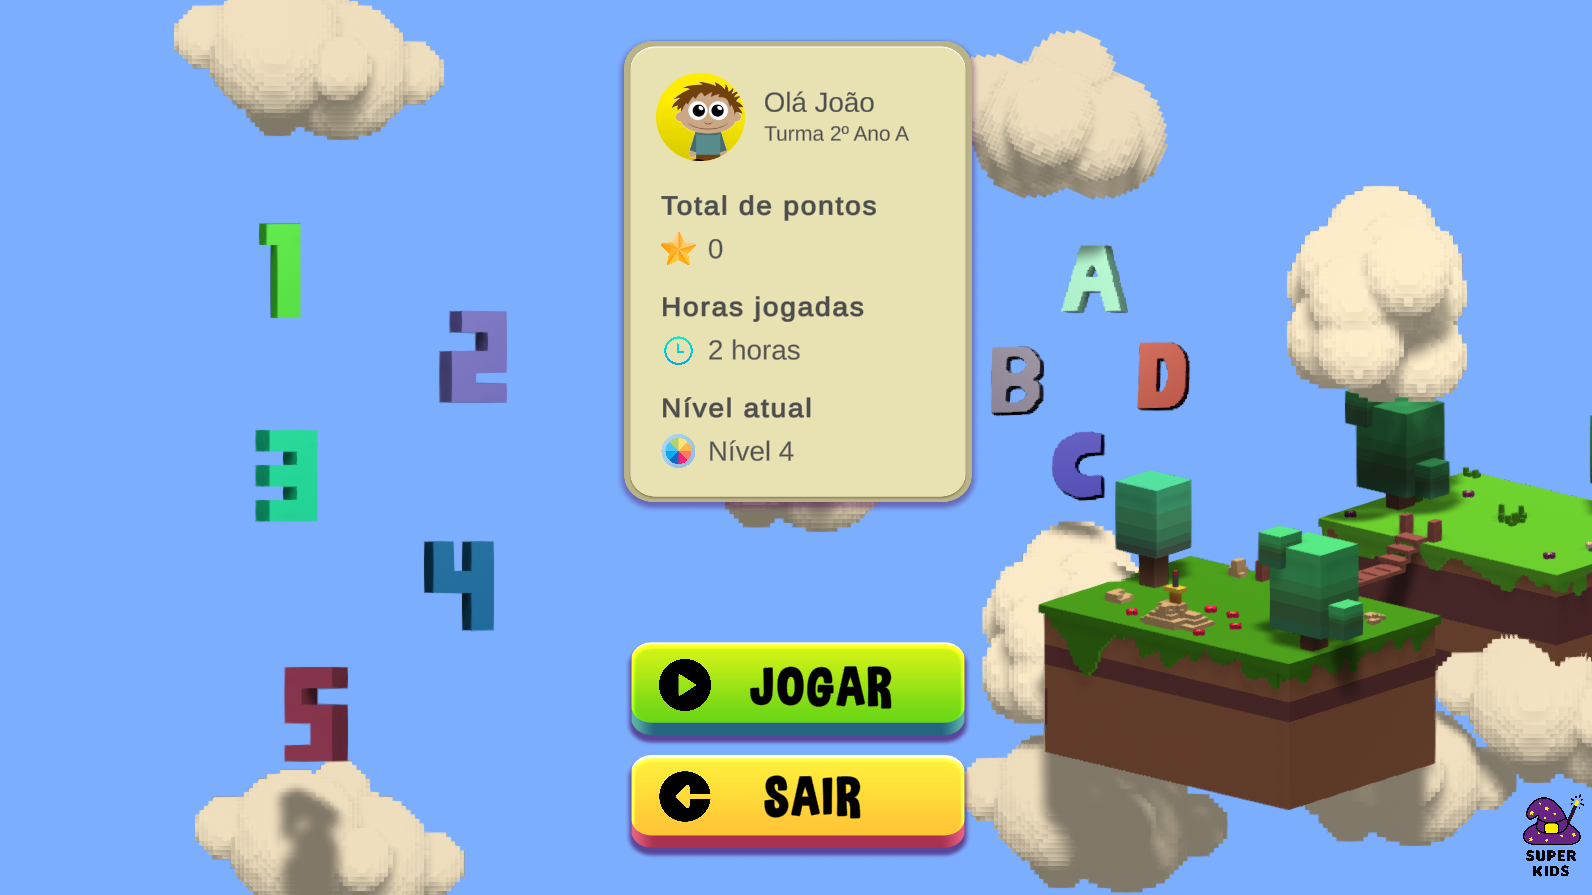
\includegraphics[width=0.8\linewidth]{GameScreenshots/Home.png}
    \fonte{Elaborado pelo autor.}
\end{figure}

Na tela inicial (Figura \ref{fig:tela_inicial}) também é apresentado algumas informações básicas do jogador, como seu nome, série que está cursando, nível atual e o seu total de pontos adquiridos ao decorrer das fases, representados por estrelas.

%%%%%%%%%%%%%%%%%%%%%%%%%%%%%%%%%%%%%%%%%%%%%%%%%%%%%%%%%%%%%%%%%%%%%%%%%%%%%
%	Tela de escolha de nível
%%%%%%%%%%%%%%%%%%%%%%%%%%%%%%%%%%%%%%%%%%%%%%%%%%%%%%%%%%%%%%%%%%%%%%%%%%%%%
\begin{figure}[H]
    \centering
    \caption{Tela de escolha de nível}
    \label{fig:tela_escolha_nivel}
    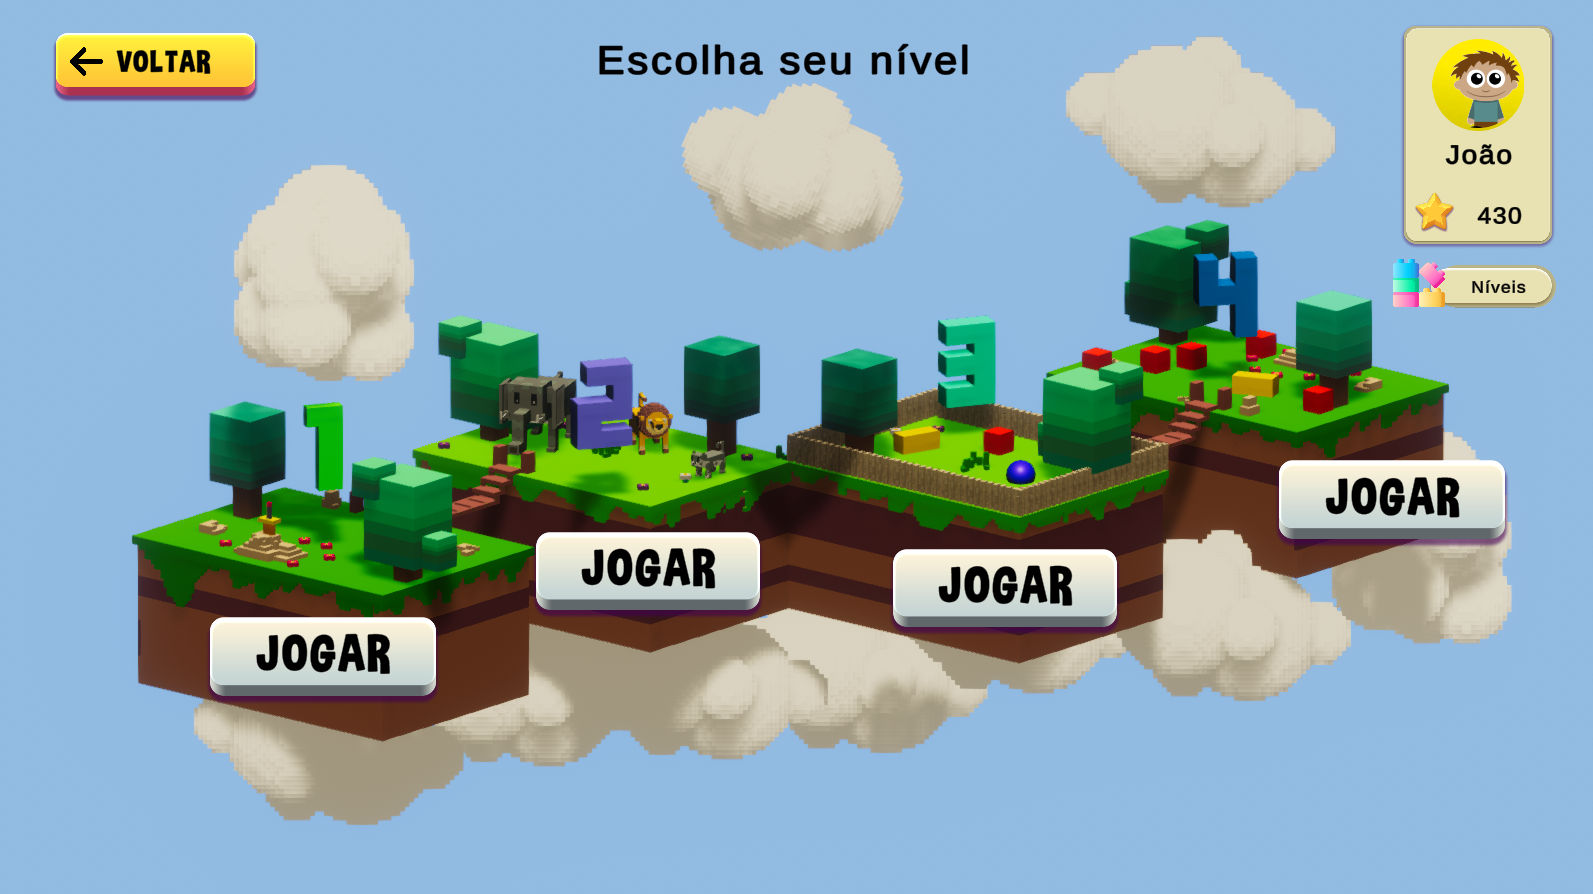
\includegraphics[width=0.8\linewidth]{GameScreenshots/ChooseLevel.png}
    \fonte{Elaborado pelo autor.}
\end{figure}

Na tela de escolha de nível (Figura \ref{fig:tela_escolha_nivel}), estão todos os níveis disponíveis para o usuário jogar. Cada nível possui o seu botão "Jogar" que redireciona para a respectiva fase, além do botão de "Voltar" que voltará para a tela inicial.

%%%%%%%%%%%%%%%%%%%%%%%%%%%%%%%%%%%%%%%%%%%%%%%%%%%%%%%%%%%%%%%%%%%%%%%%%%%%%
%	NÍVEL 1
%%%%%%%%%%%%%%%%%%%%%%%%%%%%%%%%%%%%%%%%%%%%%%%%%%%%%%%%%%%%%%%%%%%%%%%%%%%%%
\begin{figure}[H]
    \centering
    \caption{Nível 1}
    \label{fig:nivel_1}
    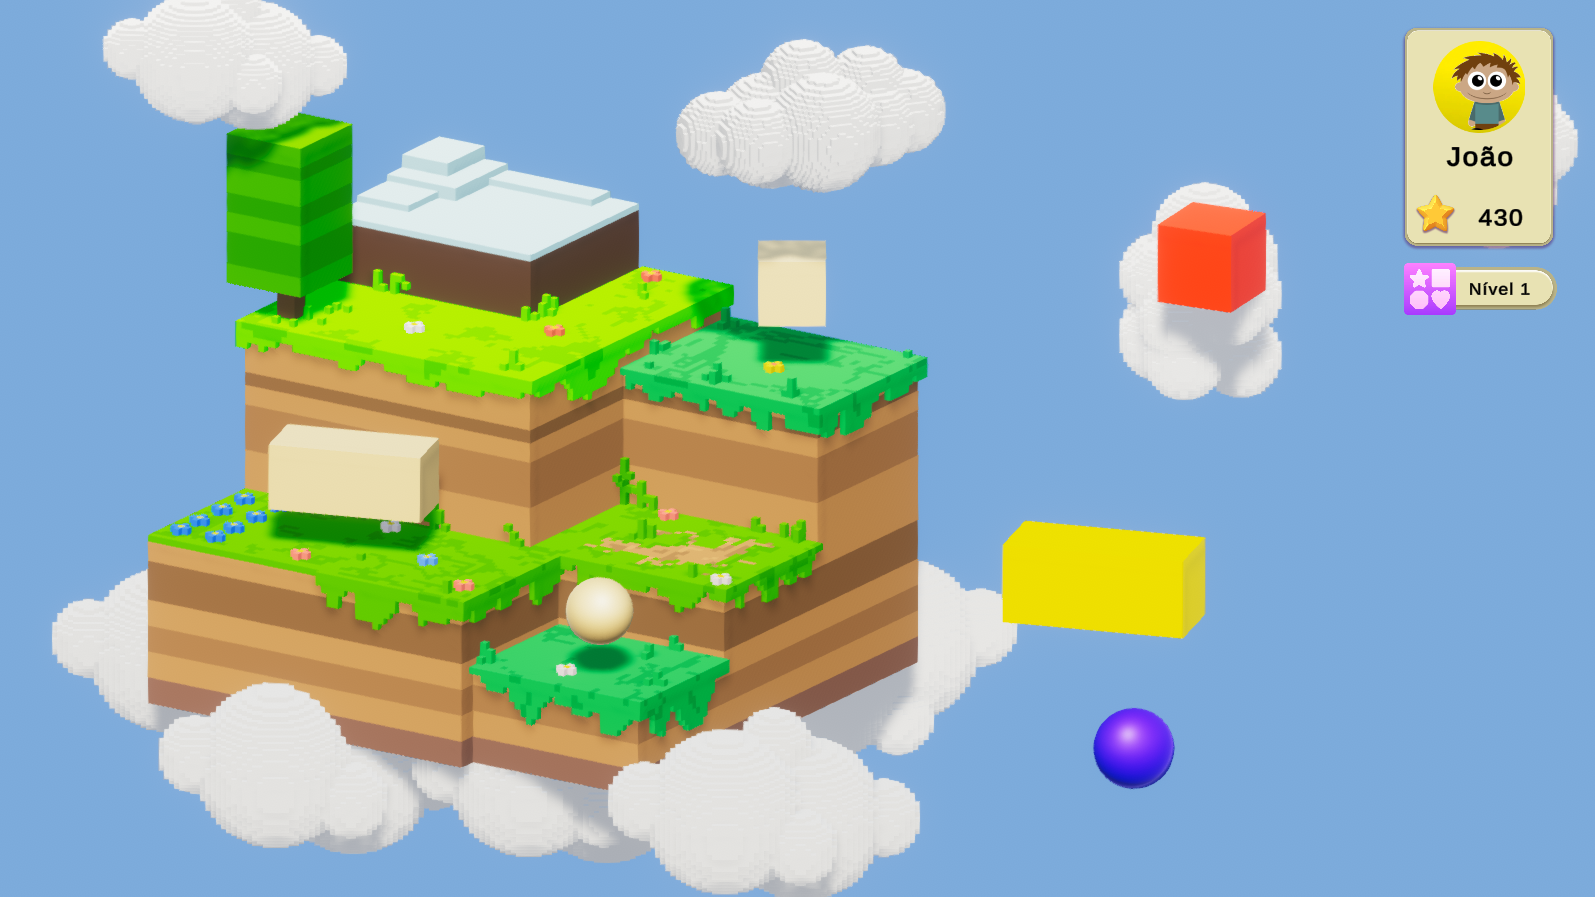
\includegraphics[width=0.8\linewidth]{GameScreenshots/Level1.png}
    \fonte{Elaborado pelo autor.}
\end{figure}

O nível 1 (Figura \ref{fig:nivel_1}) aborda sobre as formas geométricas, tendo como objetivo encaixar as formas nos seus respectivos espaços presentes na ilha flutuante.

O jogador clica sob a forma e arrasta-a para a posição a qual julgar correta na ilha, para assim tentar encaixá-la. Caso seja colocado na posição certa, será emitido um som e exibido uma mensagem, acontecendo o mesmo caso o jogador erre. Este mesmo comportamento é aplicado a todos os outros níveis após a resposta e/ou ação do jogador.

Assim que o jogador encaixa todas as 3 formas aparecerá uma janela (Figura \ref{fig:nivel_1_concluido}) parabenizando-o e com os botões de “Próxima fase”, redirecionando para o próximo nível, "Jogar novamente", reiniciando o nível, e "Voltar", voltando a tela de escolha de níveis (Figura \ref{fig:tela_escolha_nivel}). Está mesma janela está presente em todos os outros nível quando finalizados.

\begin{figure}[H]
    \centering
    \caption{Janela de exibida ao completar o nível 1}
    \label{fig:nivel_1_concluido}
    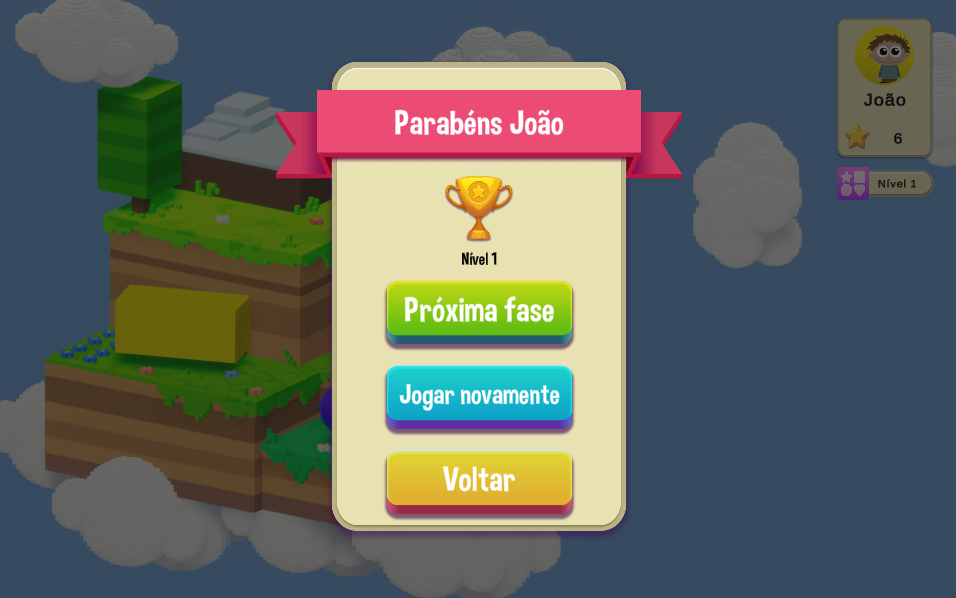
\includegraphics[width=0.8\linewidth]{GameScreenshots/Win.png}
    \fonte{Elaborado pelo autor.}
\end{figure}

Por fim, para o nível 1 (Figura \ref{fig:nivel_1}) foi levado em consideração os \textbf{Objetivos de aprendizagem e desenvolvimento para a educação infantil}, como o objetivo \textbf{EI03ET01}, o qual propõe o estabelecimento de comparações entre objetos levando em consideração suas propriedades (como cor e tamanho).

\begin{figure}[H]
    \centering
    \caption{Nível 2}
    \label{fig:nivel_2}
    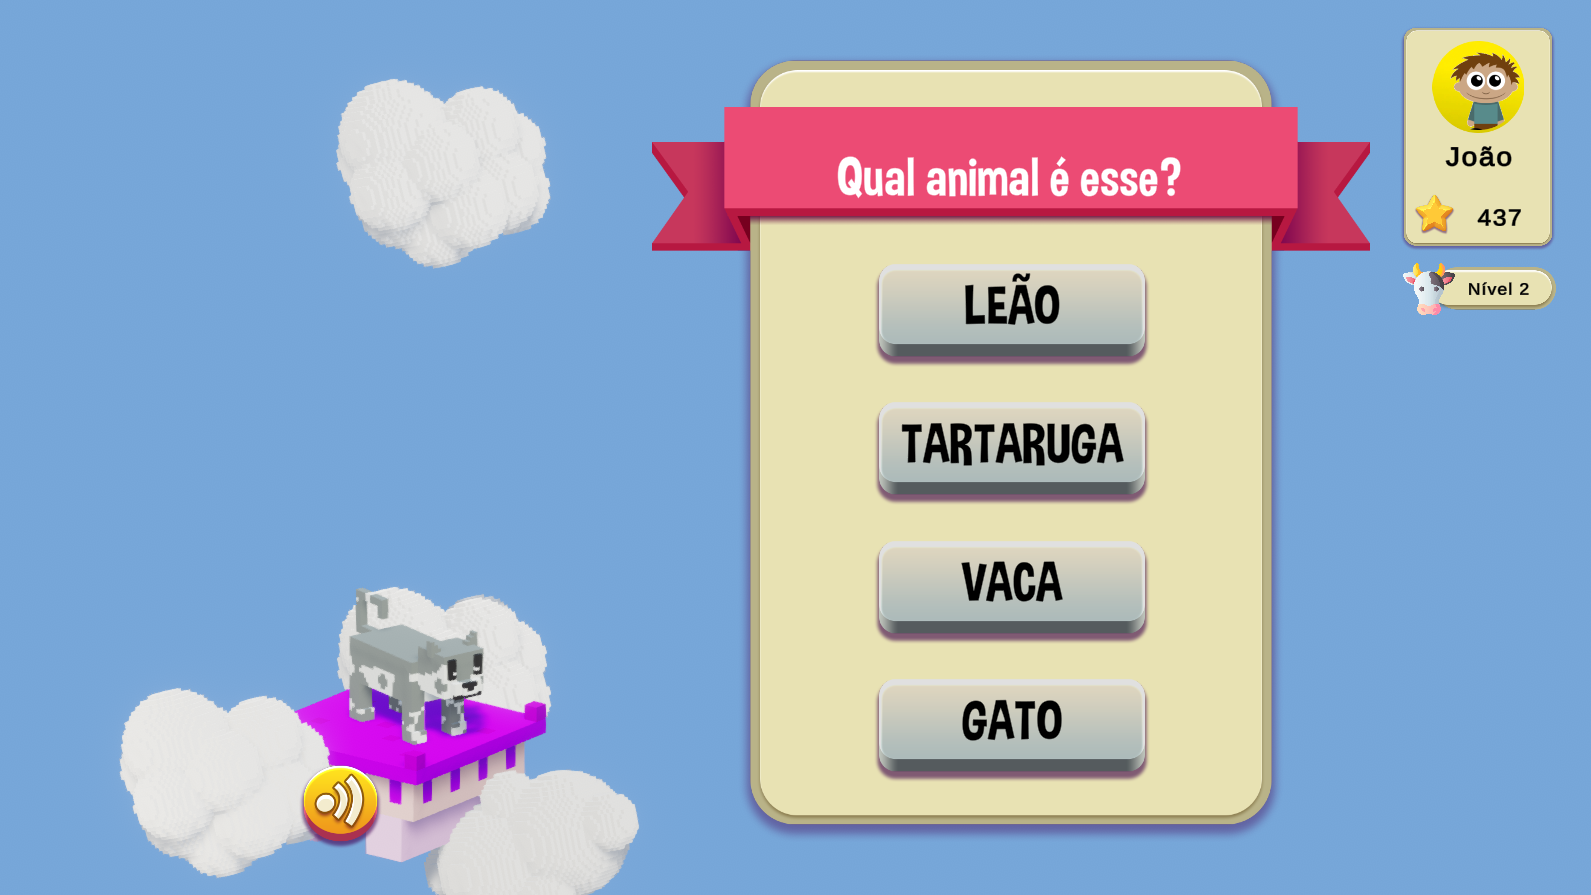
\includegraphics[width=0.8\linewidth]{GameScreenshots/Level2.png}
    \fonte{Elaborado pelo autor.}
\end{figure}

O nível 2 (Figura \ref{fig:nivel_2}) diz respeito a relação dos sons com os respectivos animais, objetivando a escolha correta dentre as opções exibidas na tela de acordo com o animal que está sendo apresentado e o seu som.

Para este nível o objetivo de aprendizagem levado em consideração foi o \textbf{EI03TS01}, o qual visa a utilização de sons produzidos por materiais, objetos e instrumentos nas brincadeiras de faz de conta e outras atividades lúdicas.

\begin{figure}[H]
    \centering
    \caption{Nível 3}
    \label{fig:nivel_3}
    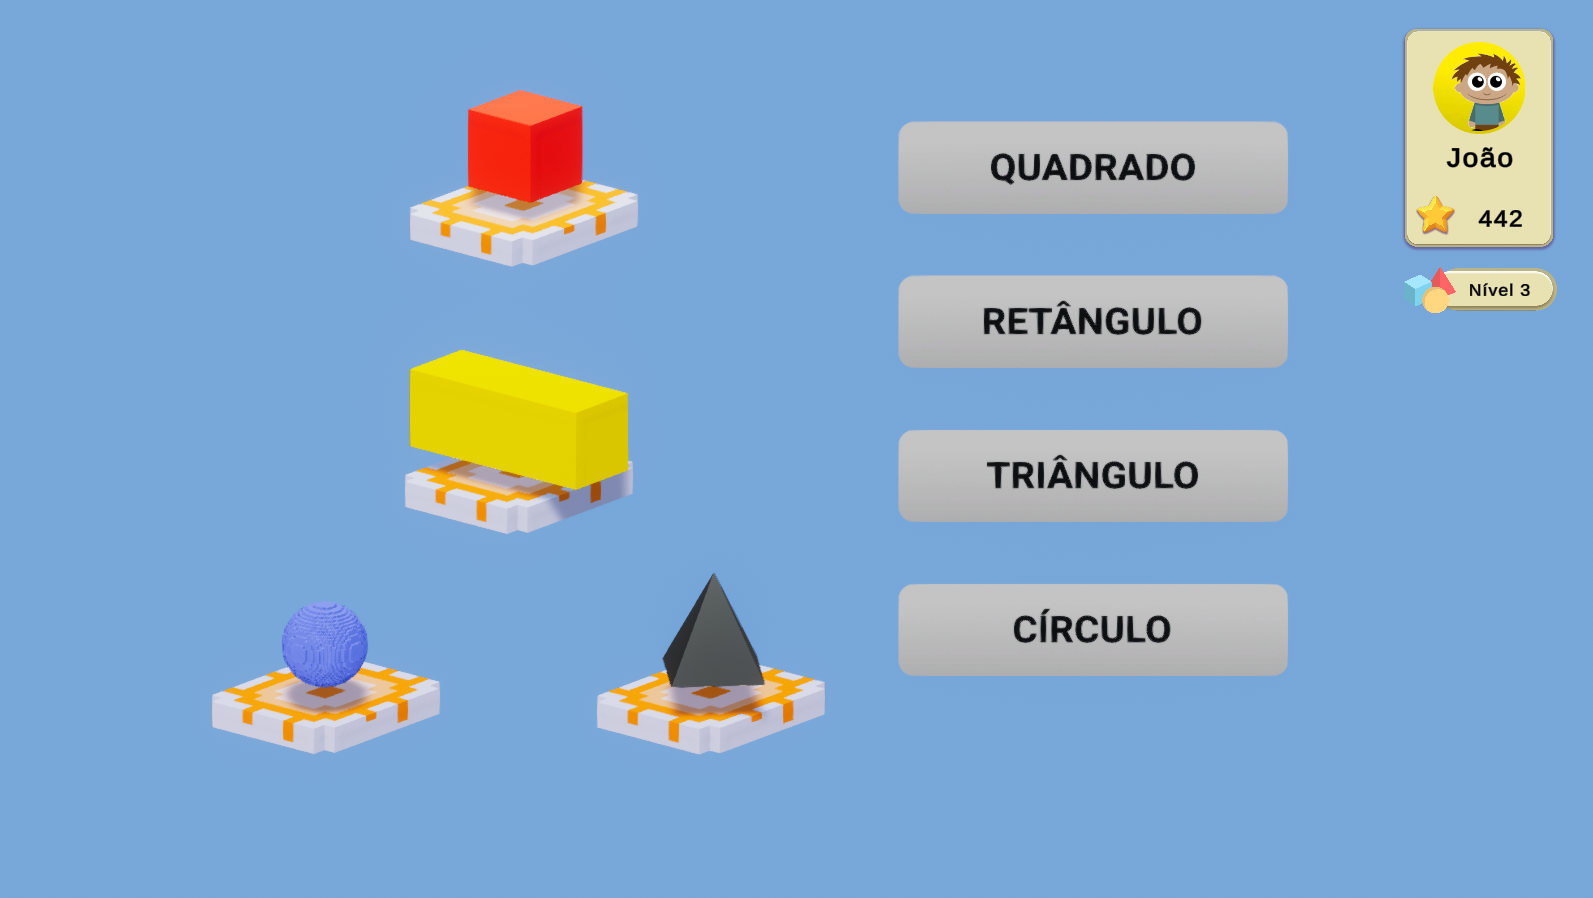
\includegraphics[width=0.8\linewidth]{GameScreenshots/Level3.png}
    \fonte{Elaborado pelo autor.}
\end{figure}

Já o nível 3 (Figura \ref{fig:nivel_3}) aborda sobre a classificação das respectivas formas geométricas e seus nomes, no qual usuário deverá clicar e arrastar o nome até próximo da forma geométrica desejada.

Para esse nível o objetivo de aprendizagem aplicado foi o \textbf{EI03ET05}, o qual propõe a classificação de objetos e figuras de acordo com as suas semelhanças e diferenças.

\begin{figure}[H]
    \centering
    \caption{Nível 4}
    \label{fig:nivel_4}
    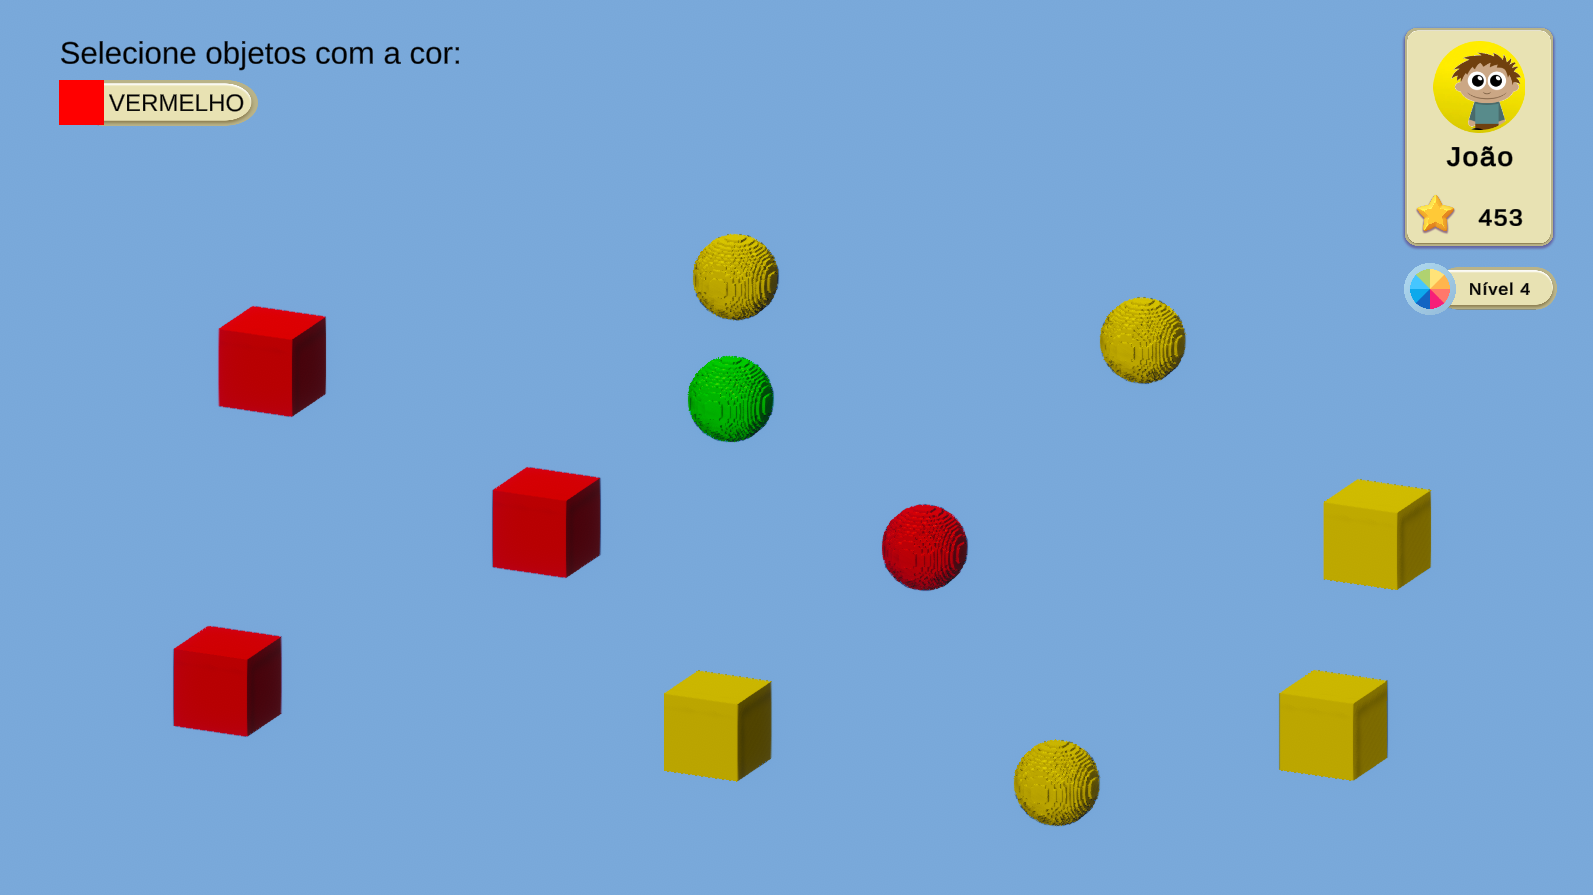
\includegraphics[width=0.8\linewidth]{GameScreenshots/Level4.png}
    \fonte{Elaborado pelo autor.}
\end{figure}

Por fim, o nível 4 (Figura \ref{fig:nivel_4}) também aborda sobre as formas geométricas, contudo tendo como objetivo a seleção e diferenciação das cores dos objetos apresentados, onde o usuário clicará em cima do objeto que julgar da mesma cor da pedida pelo nível.

Assim sendo, utilizou-se do mesmo objetivo de aprendizagem do nível 1 (Figura \ref{fig:nivel_1}), o \textbf{EI03ET01}, aplicando também o conceito de estabelecimento de comparações entre objetos levando em consideração suas propriedades, nesse caso a sua cor.

Para todos os níveis foi levado em consideração alguns campos de experiências, como o de \textbf{Corpo, gestos e movimentos} que emprega a utilização de elementos sensoriais e imaginários, brincadeiras de faz de conta, como as ilhas flutuantes em um mundo mágico e os sons de acerto, erro e dos animais utilizados no jogo.

Outro campo aplicado foi o \textbf{Traço, sons, cores e formas} aplicando-se a manipulação e exploração dos recursos tecnológicos, como o mouse, teclado e computador, promovendo a participação da criança em um meio artístico, o qual é o jogo digital, assim favorecendo a criatividade da mesma.

Por último incorporou-se o campo \textbf{Espaços, tempos, quantidades, relações e transformações}, abordando principalmente a ideia dos conhecimentos matemáticos, como o reconhecimento das formas geométricas, bem como a relação de dimensões e comprimentos, por exemplo diferenciando um quadrado de um retângulo.

\subsection{Aplicação da pesquisa de campo}
\label{sc:aplicacao_pesquisa}

Para a avaliação do presente projeto utilizou-se do método de pesquisa de campo, sendo a mesma feita por meio de formulários Google Forms.

A pesquisa objetivou 2 públicos diferentes, um sendo o de profissionais da área da educação e outro o público em geral, visando a validação dos conceitos aplicados aos níveis do jogo outrora apresentados no item \ref{sc:telas_jogo} deste documento. Sendo assim, a pesquisa foi realizada com 40 pessoas, sendo destas 12 profissionais da educação, utilizando as perguntas do Anexo 1 (\ref{sc:anexo1}), e 28 do público geral, apresentando as perguntas do Anexo 2 (\ref{sc:anexo2}).

\subsection{Resultados das pesquisas dos profissionais da área da educação}
\label{sc:resultados_pesquisa_professores}

Objetivou-se primeiramente entender como os profissionais enxergavam os jogos virtuais educativos como ferramenta de ensino, percebeu-se que, unanimemente, são vistos como benéficos, desde que sigam parâmetros que o validem cientificamente e que sejam bem estruturados, assim ganhando bastante aprovação.

\begin{figure}[H]
    \centering
    \caption{Professores - Pergunta 1}
    \label{fig:professor_pergunta_1}
    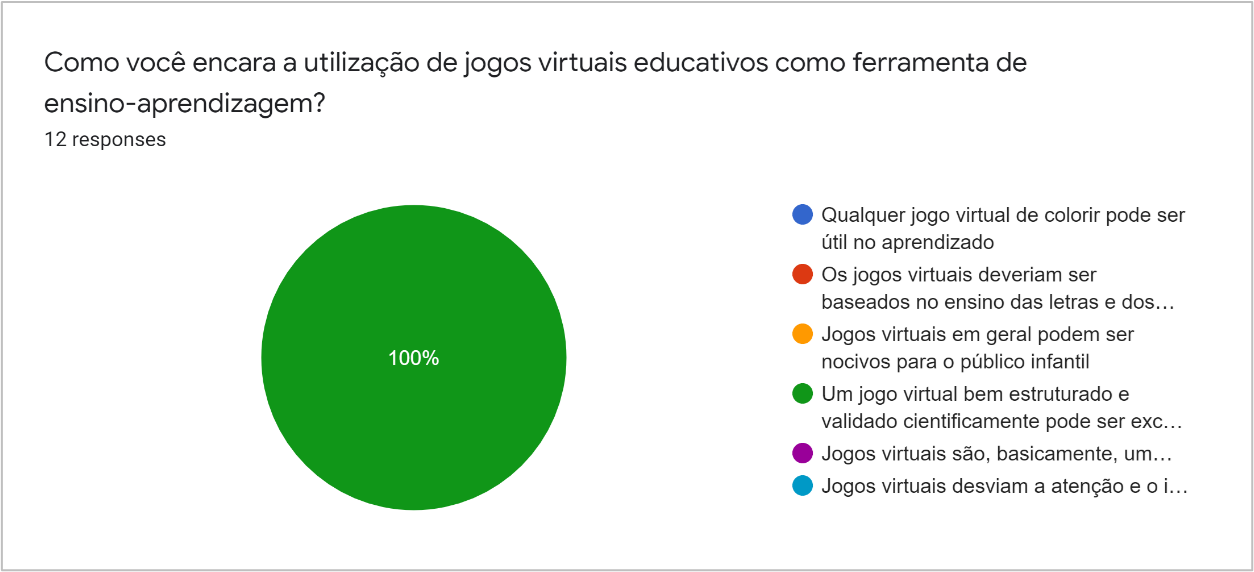
\includegraphics[width=0.8\linewidth]{SearchResults/Teachers/GamesUtilization.png}
    \fonte{Elaborado pelo autor.}
\end{figure}

Também buscou verificar se os níveis desenvolvidos na solução de software proposta atendiam os conceitos, finalidades e objetivos preconizados pela BNCC, contudo buscando uma avaliação mais pedagógica. Por fim identificou-se que a fase em questão, nível 1 (Figura \ref{fig:nivel_1}), é sim capaz de atender e utilizar dos conceitos da BNCC, tendo a média de avaliações entre 4 e 5.

\begin{figure}[H]
    \centering
    \caption{Professores - Pergunta 2}
    \label{fig:professor_pergunta_2}
    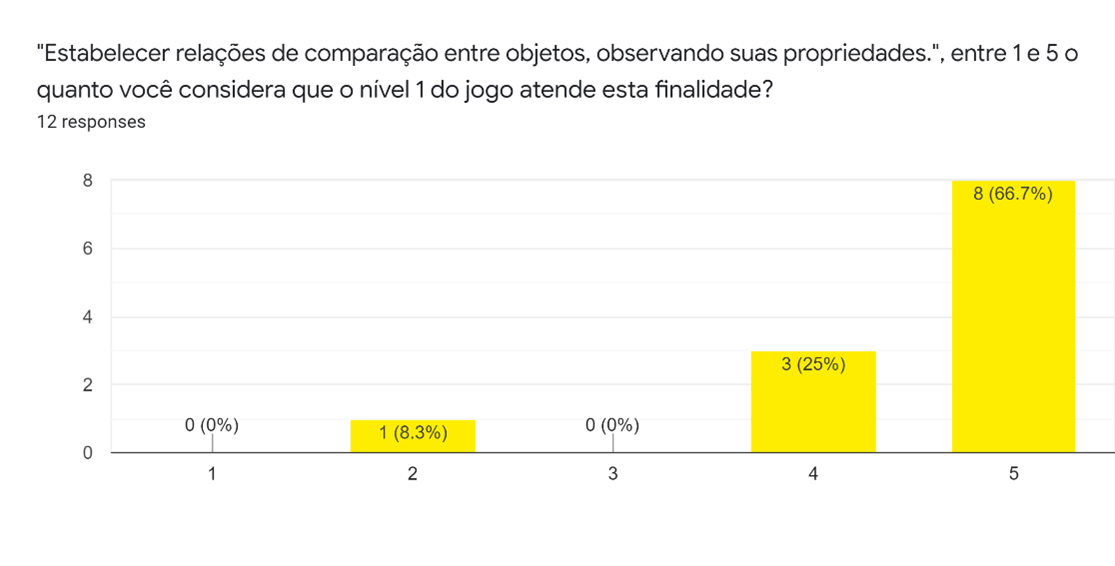
\includegraphics[width=0.8\linewidth]{SearchResults/Teachers/Level1.png}
    \fonte{Elaborado pelo autor.}
\end{figure}

Assim como a pergunta sobre o nível 1 (Figura \ref{fig:professor_pergunta_2}), para a pergunta a respeito do nível 2 (Figura \ref{fig:professor_pergunta_3}) buscou-se o mesmo objetivo, tendo também um resultado satisfatório, visto que a fase utilizava sim de recursos sonoros, todavia não exatamente os mesmos contidos na BNCC.

\begin{figure}[H]
    \centering
    \caption{Professores - Pergunta 3}
    \label{fig:professor_pergunta_3}
    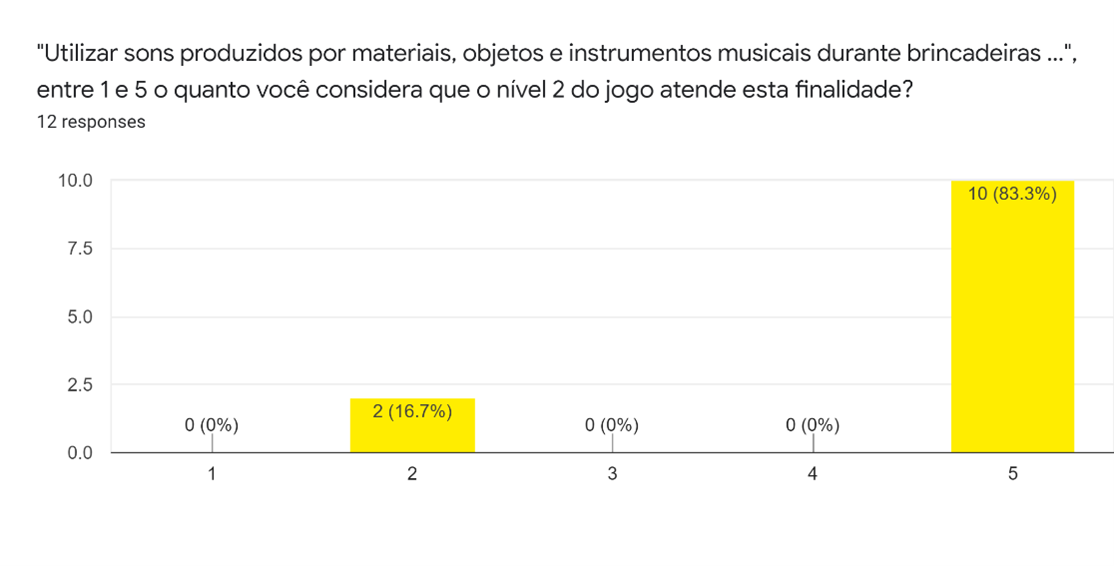
\includegraphics[width=0.8\linewidth]{SearchResults/Teachers/Level2.png}
    \fonte{Elaborado pelo autor.}
\end{figure}

\subsection{Resultados das pesquisas do público geral}
\label{sc:resultados_pesquisa_publico}

A fim de verificar qual a opinião do público geral a respeito de metodologias que utilizam recursos lúdicos, observou-se que a utilização de tais recursos no quesito ensino-aprendizagem, agregados a metodologias, vem obtendo cada vez mais reconhecimento, logo sendo uma possível porta de entrada para o uso de jogos virtuais educativos em sala de aula.

\begin{figure}[H]
    \centering
    \caption{Público geral - Pergunta 1}
    \label{fig:aluno_pergunta_1}
    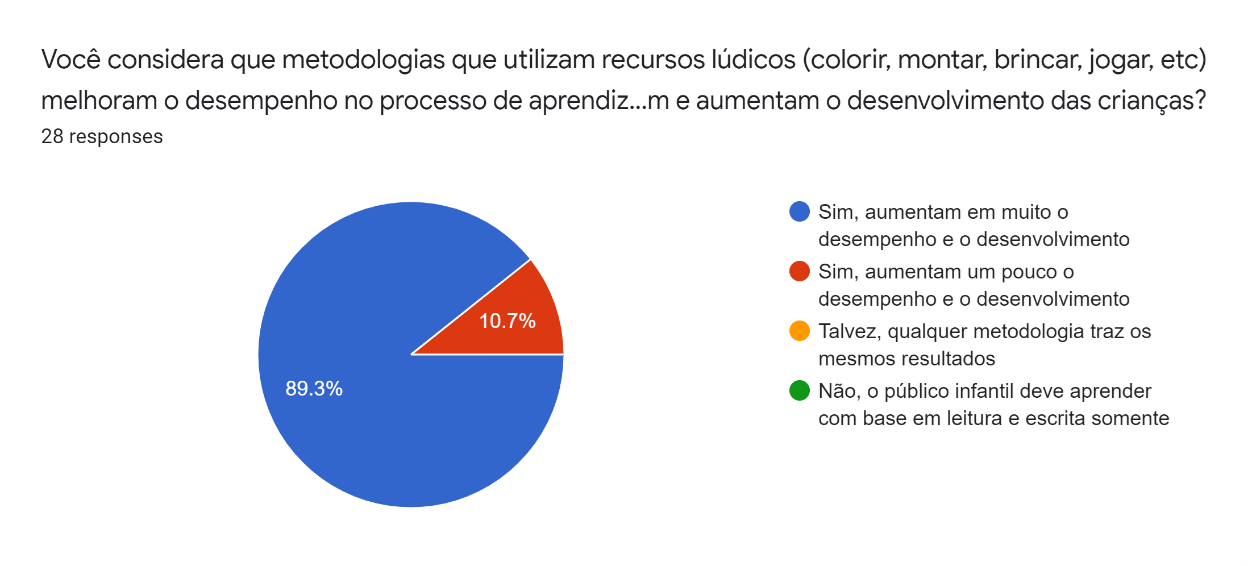
\includegraphics[width=0.8\linewidth]{SearchResults/Students/LudicMetodologies.png}
    \fonte{Elaborado pelo autor.}
\end{figure}

Assim como as perguntas referentes aos níveis do jogo feitas com os profissionais da educação, também se utilizou dos mesmos objetivos com o público geral, todavia visando uma visão e avaliação mais simplista das fases do jogo, a respeito do nível 3 (Figura \ref{fig:aluno_pergunta_2}), que obteve uma boa avaliação, visto que a fase possibilitava sim a classificação das respectivas formas exibidas.

\begin{figure}[H]
    \centering
    \caption{Público geral - Pergunta 2}
    \label{fig:aluno_pergunta_2}
    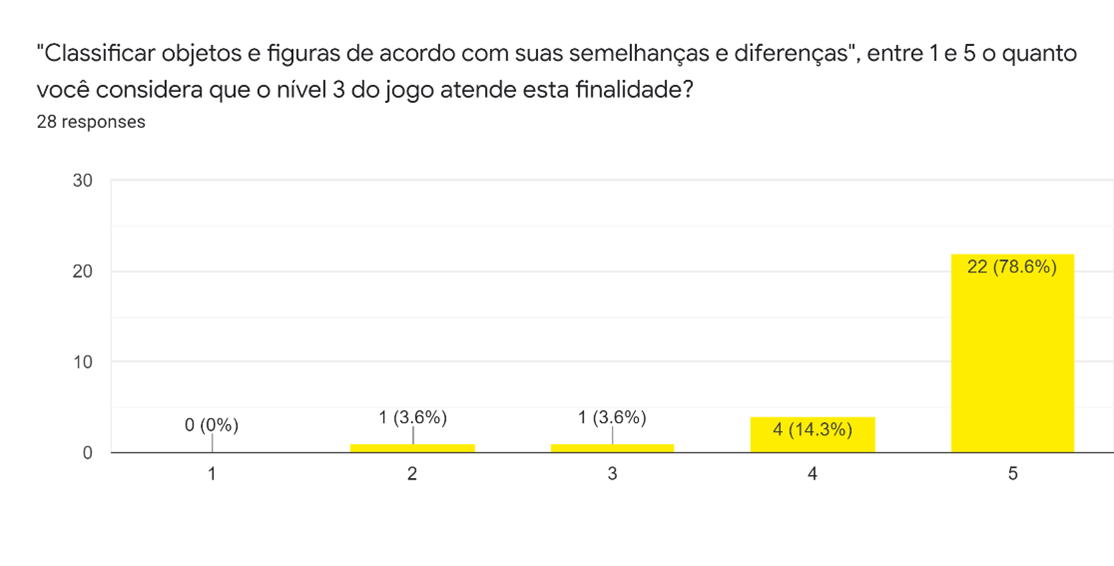
\includegraphics[width=0.8\linewidth]{SearchResults/Students/Level3.png}
    \fonte{Elaborado pelo autor.}
\end{figure}

Tal como as perguntas posteriores as quais dizem respeito as avaliações dos níveis, teve pôr fim a avaliação da última fase do jogo, sobre o nível 4 (Figura \ref{fig:aluno_pergunta_3}), tendo também um resultado bastante satisfatório, sendo que na mesma é sim possível a relação de comparação entre os objetos pelas suas cores.

\begin{figure}[H]
    \centering
    \caption{Público geral - Pergunta 3}
    \label{fig:aluno_pergunta_3}
    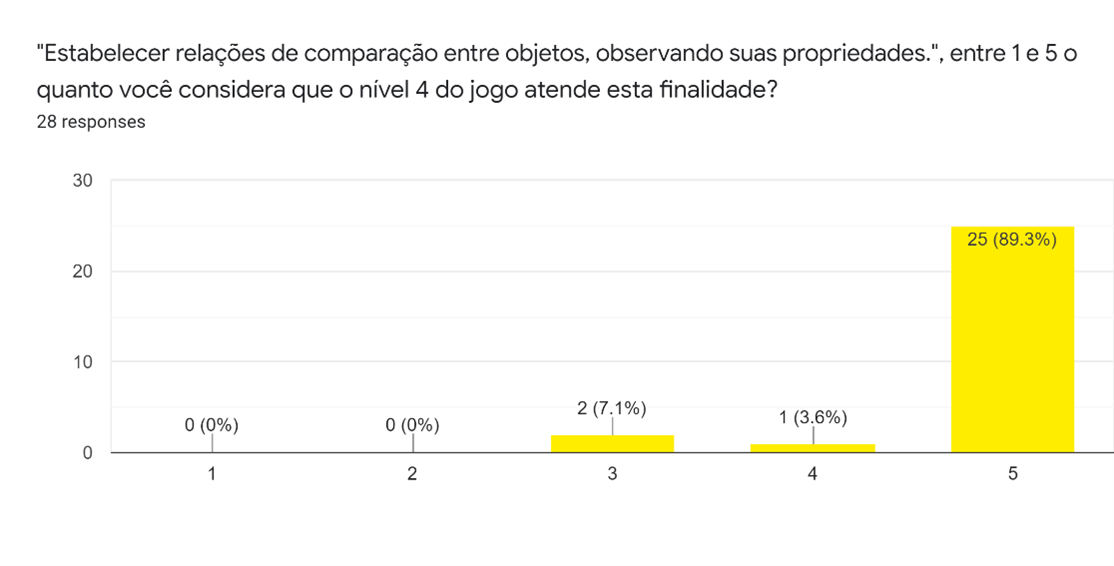
\includegraphics[width=0.8\linewidth]{SearchResults/Students/Level4.png}
    \fonte{Elaborado pelo autor.}
\end{figure}

%%%%%%%%%%%%%%%%%%%%%%%%%%%%%%%%%%%%%%%%%%%%%%%%%%%%%%%%%%%%%%%%%%%%%%%%%%%%%
%	CONCLUSÃO
%%%%%%%%%%%%%%%%%%%%%%%%%%%%%%%%%%%%%%%%%%%%%%%%%%%%%%%%%%%%%%%%%%%%%%%%%%%%%
\section{Conclusão}
\label{sc:conclusao}

Com base no jogo desenvolvido e nos dados obtidos nos itens \ref{sc:resultados_pesquisa_professores} e \ref{sc:resultados_pesquisa_publico} deste documento, este projeto apresentou uma solução de tecnologia em forma de jogo virtual educativo o qual visa ser ator coadjuvante no processo ensino-aprendizagem, auxiliando o professor em sala de aula, com base em documentos norteadores oficiais.

Percebeu-se que, nas pesquisas de campo realizadas, houve um maior consenso entre os profissionais da educação na grande maioria das respostas coletas, logo sendo um ótimo indicativo da aplicação e validação pedagógica/científica do projeto.

Dessarte, ainda sobre as pesquisas realizadas, atestou-se a possível utilização ou recomendação de um jogo virtual educativo como ferramenta complementar a aula sendo muito alta, bem como a consideração do mesmo como uma poderosa ferramenta para o processo ensino-aprendizagem, desde que haja os devidos monitoramentos e limites.

Conclui-se assim que os jogos virtuais educativos quando bem estruturados e desenvolvidos, utilizando de documentos norteadores oficiais de acordo com nosso atual sistema de ensino e recursos lúdicos, são ferramentas poderosas que prendem a atenção do usuário ao objetivo do jogo, logo desenvolvendo suas funções cognitivas e educacionais.

Como possíveis trabalhos futuros pretende-se, em primeiro lugar, implementar tutoriais de jogabilidade aos níveis do jogo, identificando as ações iniciais a serem feitas de cada nível e, caso o usuário esteja a muito tempo em dúvida, dar dicas visuais da ação a ser tomada.

Em segundo lugar deseja-se realizar diversos testes e pesquisas qualitativas e quantitativas, utilizando uma versão \textit{alpha} do jogo, aplicando os mesmos níveis em instituições de rede pública e privada, visando comparar e acompanhar junto ao público-alvo os respectivos resultados, posteriormente evidenciando possíveis discrepâncias no ensino e suas causas, além de avaliar a jogabilidade e usabilidade no geral.

Por fim, pretende-se realizar entrevistas com psicopedagogos, psicólogos e pedagogos a respeito de recursos, metodologias, técnicas etc. a serem implementados, como paletas de cores, personagens, desafios, dentre outros objetos e conceitos condizentes com o contexto infantil.


%%%%%%%%%%%%%%%%%%%%%%%%%%%%%%%%%%%%%%%%%%%%%%%%%%%%%%%%%%%%%%%%%%%%%%%%%%%%%
%	REFERÊNCIAS BIBLIOGRÁFICAS
%%%%%%%%%%%%%%%%%%%%%%%%%%%%%%%%%%%%%%%%%%%%%%%%%%%%%%%%%%%%%%%%%%%%%%%%%%%%%
\bibliography{references}

\section{Anexo 1 - Perguntas para o público geral}
\label{sc:anexo1}

\textbf{Pergunta 1} - Você considera que metodologias que utilizam recursos lúdicos (colorir, montar, brincar, jogar, etc.) melhoram o desempenho no processo de aprendizagem e aumentam o desenvolvimento das crianças?
\begin{itemize}
     \item Sim, aumentam em muito o desempenho e o desenvolvimento
     \item Sim, aumentam um pouco o desempenho e o desenvolvimento
     \item Talvez, qualquer metodologia traz os mesmos resultados
     \item Não, o público infantil deve aprender com base em leitura e escrita somente
\end{itemize}

\textbf{Pergunta 2} - Escolha a seguir apenas 3 atividades que você acha que podem mais impulsionar o aprendizado infantil na escola:
\begin{todolist}
     \item Uso de massinha de modelar
     \item Confecção de desenhos
     \item Colorir pinturas
     \item Relacionar itens com características em comum
     \item Treinar o alfabeto de forma escrita
     \item Brincar com objetos em formatos geométricos, de letras e números
     \item Brincar com objetos de diferentes formatos e cores
     \item Aprender músicas infantis
     \item Decorar letras e números
\end{todolist}

\textbf{Pergunta 3} - Como você encara a utilização de jogos virtuais educativos como ferramenta de ensino?
\begin{itemize}
     \item Qualquer jogo virtual  de colorir pode ser útil no aprendizado
     \item Os jogos virtuais deveriam ser baseados no ensino das letras e dos números
     \item Jogos virtuais em geral podem ser nocivos para o público infantil
     \item Um jogo virtual  bem estruturado e validado cientificamente pode ser excelente ao processo ensino-aprendizagem
     \item Jogos virtuais são, basicamente, um meio de entretenimento
     \item Jogos virtuais desviam a atenção e o interesse da criança para os estudos e o convívio social
\end{itemize}

\textbf{Pergunta 4} - Você recomendaria a utilização de um jogo virtual educativo em sala de aula como ferramenta complementar à aula do professor?
\begin{itemize}
     \item Sim
     \item Não
\end{itemize}

\textbf{Pergunta 5} - "Estabelecer relações de comparação entre objetos, observando suas propriedades.", entre 1 e 5 o quanto você considera que o nível 1 do jogo atende esta finalidade?

\begin{figure}[H]
    \centering
    \label{fig:aluno_pergunta_5}
    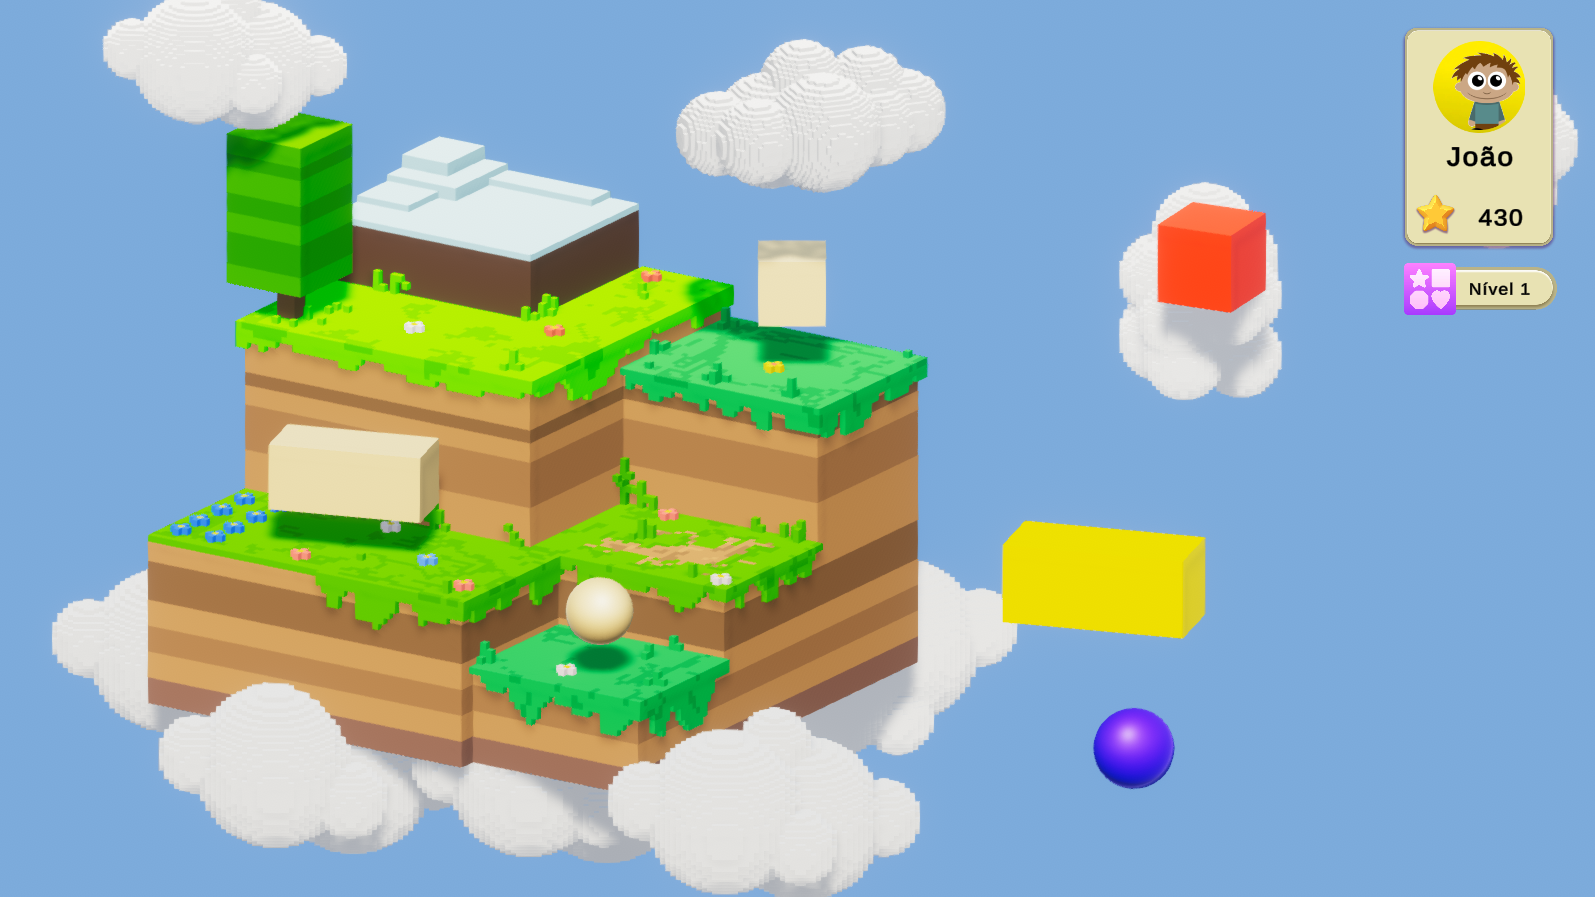
\includegraphics[width=0.8\linewidth]{GameScreenshots/Level1.png}
\end{figure}

\normalfont
\begin{tasks}[style=enumerate, item-format={\normalfont\tiny}, after-item-skip=4mm](6)
\task Não atende
\task 
\task 
\task 
\task Atende completamente
\end{tasks}

\textbf{Pergunta 6} - "Utilizar sons produzidos por materiais, objetos e instrumentos musicais durante brincadeiras ...", entre 1 e 5 o quanto você considera que o nível 2 do jogo atende esta finalidade?

\begin{figure}[H]
    \centering
    \label{fig:aluno_pergunta_5}
    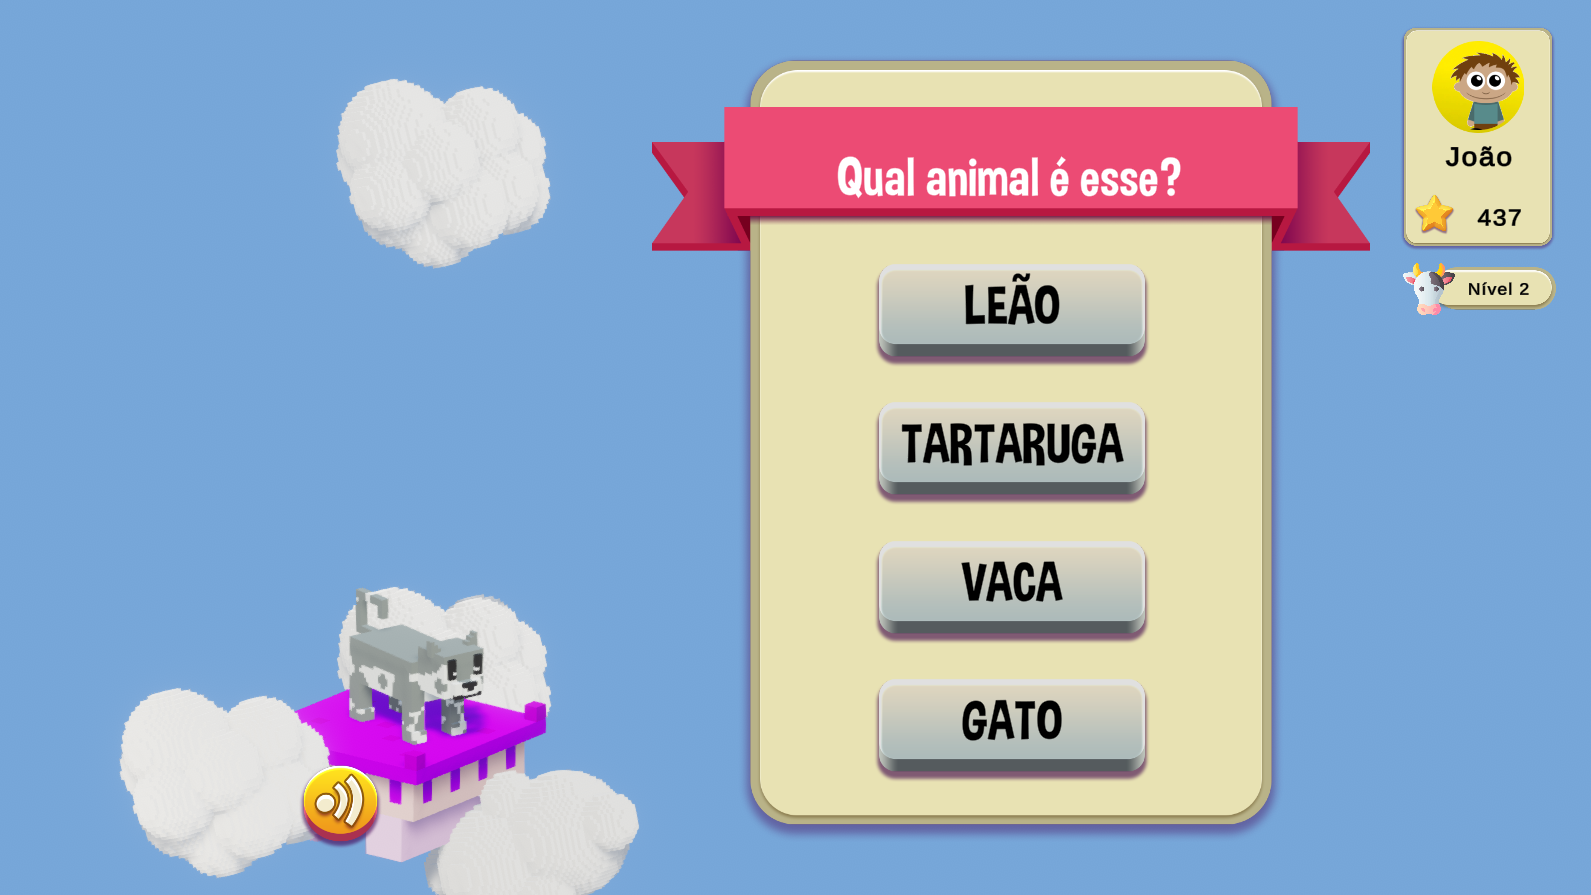
\includegraphics[width=0.8\linewidth]{GameScreenshots/Level2.png}
\end{figure}

\normalfont
\begin{tasks}[style=enumerate, item-format={\normalfont\tiny}, after-item-skip=4mm](6)
\task Não atende
\task 
\task 
\task 
\task Atende completamente
\end{tasks}

\textbf{Pergunta 7} - "Classificar objetos e figuras de acordo com suas semelhanças e diferenças", entre 1 e 5 o quanto você considera que o nível 3 do jogo atende esta finalidade?

\begin{figure}[H]
    \centering
    \label{fig:aluno_pergunta_5}
    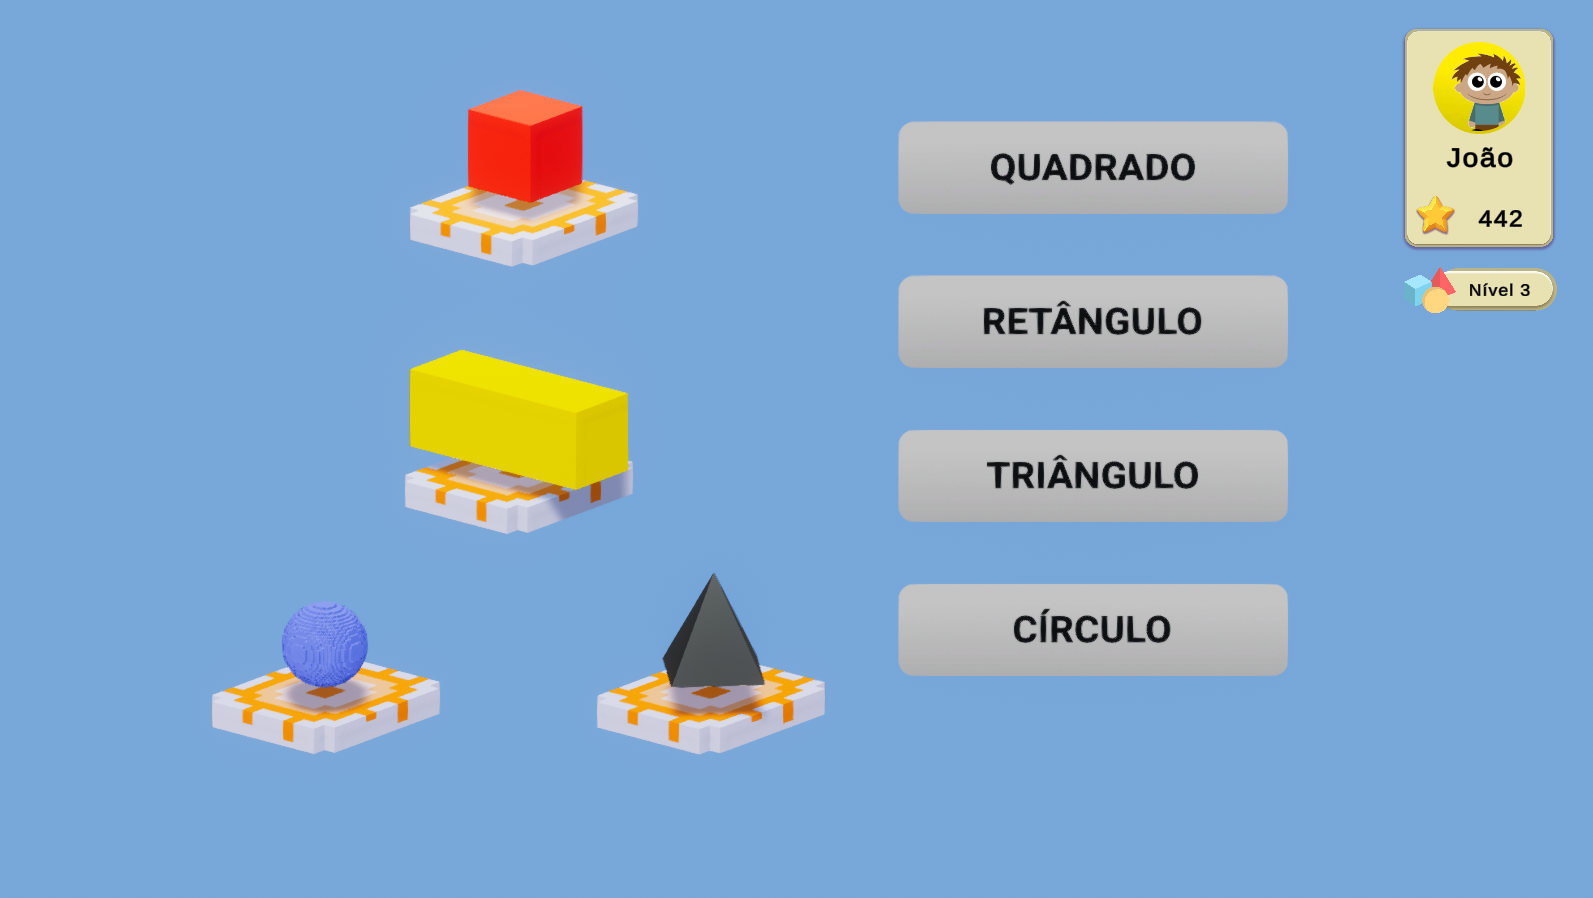
\includegraphics[width=0.8\linewidth]{GameScreenshots/Level3.png}
\end{figure}

\normalfont
\begin{tasks}[style=enumerate, item-format={\normalfont\tiny}, after-item-skip=4mm](6)
\task Não atende
\task 
\task 
\task 
\task Atende completamente
\end{tasks}

\textbf{Pergunta 8} - "Estabelecer relações de comparação entre objetos, observando suas propriedades.", entre 1 e 5 o quanto você considera que o nível 4 do jogo atende esta finalidade?

\begin{figure}[H]
    \centering
    \label{fig:aluno_pergunta_5}
    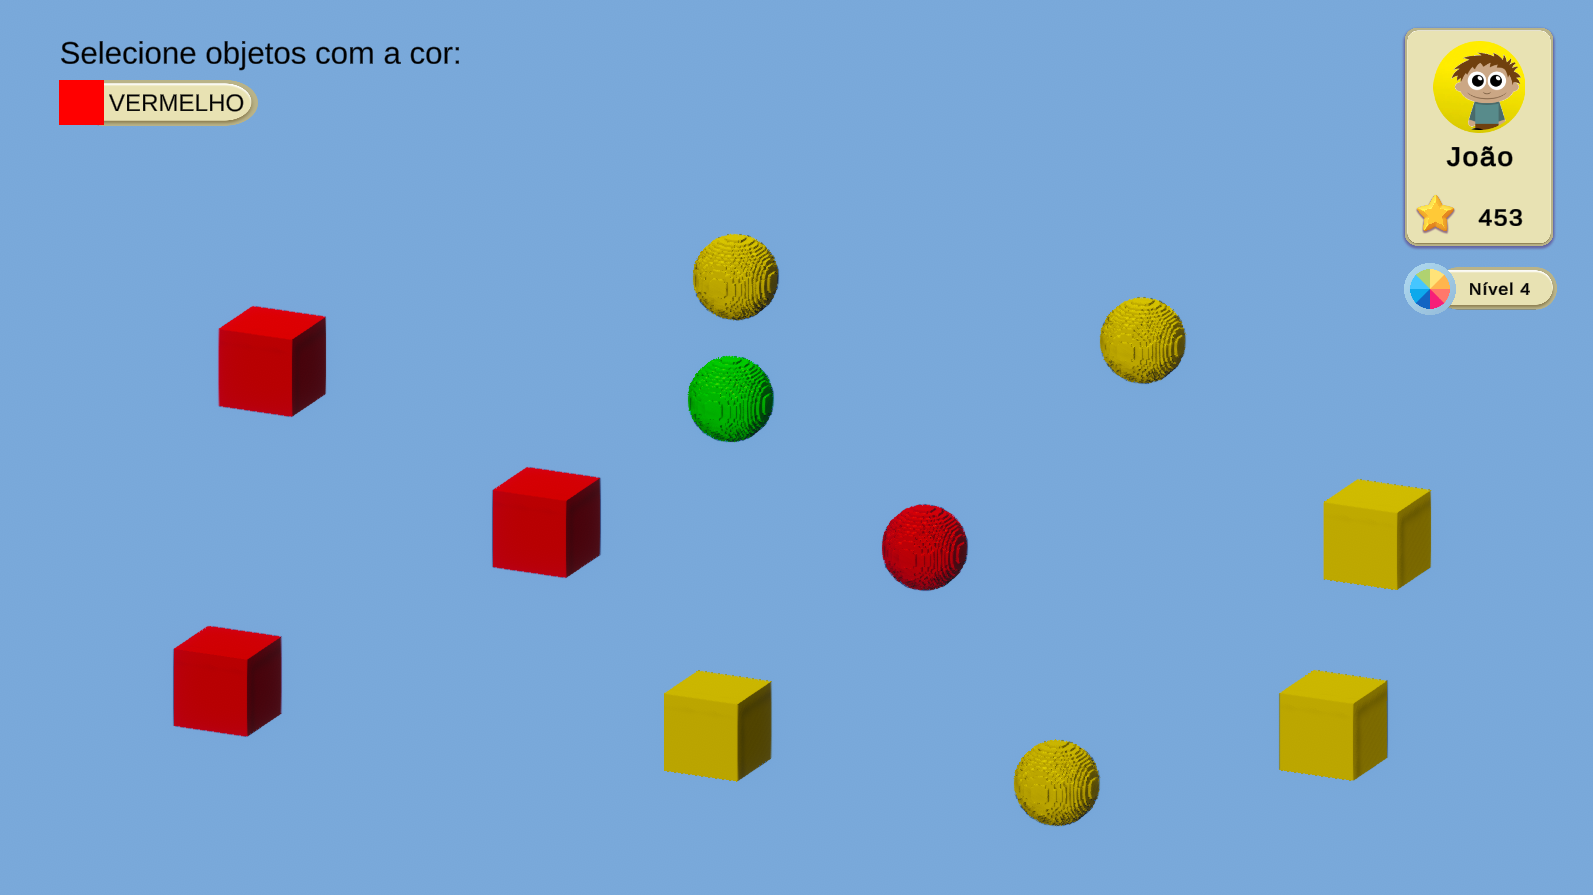
\includegraphics[width=0.8\linewidth]{GameScreenshots/Level4.png}
\end{figure}

\normalfont
\begin{tasks}[style=enumerate, item-format={\normalfont\tiny}, after-item-skip=4mm](6)
\task Não atende
\task 
\task 
\task 
\task Atende completamente
\end{tasks}

\textbf{Pergunta 9} - Na sua opinião, você acha que os jogos virtuais educativos, se utilizados com os devidos monitoramentos e limites, poderiam se tornar uma poderosa ferramenta para o processo de ensino-aprendizagem?
\begin{itemize}
     \item Sim
     \item Não
\end{itemize}

\textbf{Pergunta 10} - Se não, justifique sua resposta:

\textbf{Pergunta 11} - Deseja fazer algum comentário, observação e/ou crítica? Escreva para gente:


\section{Anexo 2 - Perguntas para os profissionais da educação}
\label{sc:anexo2}

\textbf{Pergunta 1} - Quais funções você exerce?
\begin{todolist}
     \item Professor(a)
     \item Coordenador(a) pedagógico(a)
     \item Pedagogo
     \item Psicopedagogo
     \item Administrador escolar
     \item Orientador educacional
     \item Outra...
\end{todolist}

\textbf{Pergunta 2} - Em quais destas etapas você leciona/administra ou já lecionou/administrou?
\begin{todolist}
     \item Educação Infantil
     \item Ensino Fundamental I
     \item Outra...
\end{todolist}

\textbf{Pergunta 3} - Você considera que metodologias que utilizam recursos lúdicos (colorir, montar, brincar, jogar, etc.) melhoram o desempenho no processo de aprendizagem e aumentam o desenvolvimento das crianças?
\begin{itemize}
     \item Sim, aumentam em muito o desempenho e o desenvolvimento
     \item Sim, aumentam um pouco o desempenho e o desenvolvimento
     \item Talvez, qualquer metodologia traz os mesmos resultados
     \item Não, o público infantil deve aprender com base em leitura e escrita somente
\end{itemize}

\textbf{Pergunta 4} - Você considera que jogos virtuais educativos podem contribuir como mecanismo complementar e coadjuvante no processo ensino aprendizagem pela sua ludicidade?
\begin{itemize}
     \item Sim, podem contribuir em muito
     \item Sim, podem contribuir um pouco
     \item Não, sem qualquer contribuição
\end{itemize}

\textbf{Pergunta 5} - Como você encara a utilização de jogos virtuais educativos como ferramenta de ensino-aprendizagem?
\begin{itemize}
     \item Qualquer jogo virtual de colorir pode ser útil no aprendizado
     \item Os jogos virtuais deveriam ser baseados no ensino das letras e dos números
     \item Jogos virtuais em geral podem ser nocivos para o público infantil
     \item Um jogo virtual bem estruturado e validado cientificamente pode ser excelente ao processo ensino-aprendizagem
     \item Jogos virtuais são, basicamente, um meio de entretenimento
     \item Jogos virtuais desviam a atenção e o interesse da criança para os estudos e o convívio social
\end{itemize}

\textbf{Pergunta 6} - "Estabelecer relações de comparação entre objetos, observando suas propriedades.", entre 1 e 5 o quanto você considera que o nível 1 do jogo atende esta finalidade?

\begin{figure}[H]
    \centering
    \label{fig:aluno_pergunta_5}
    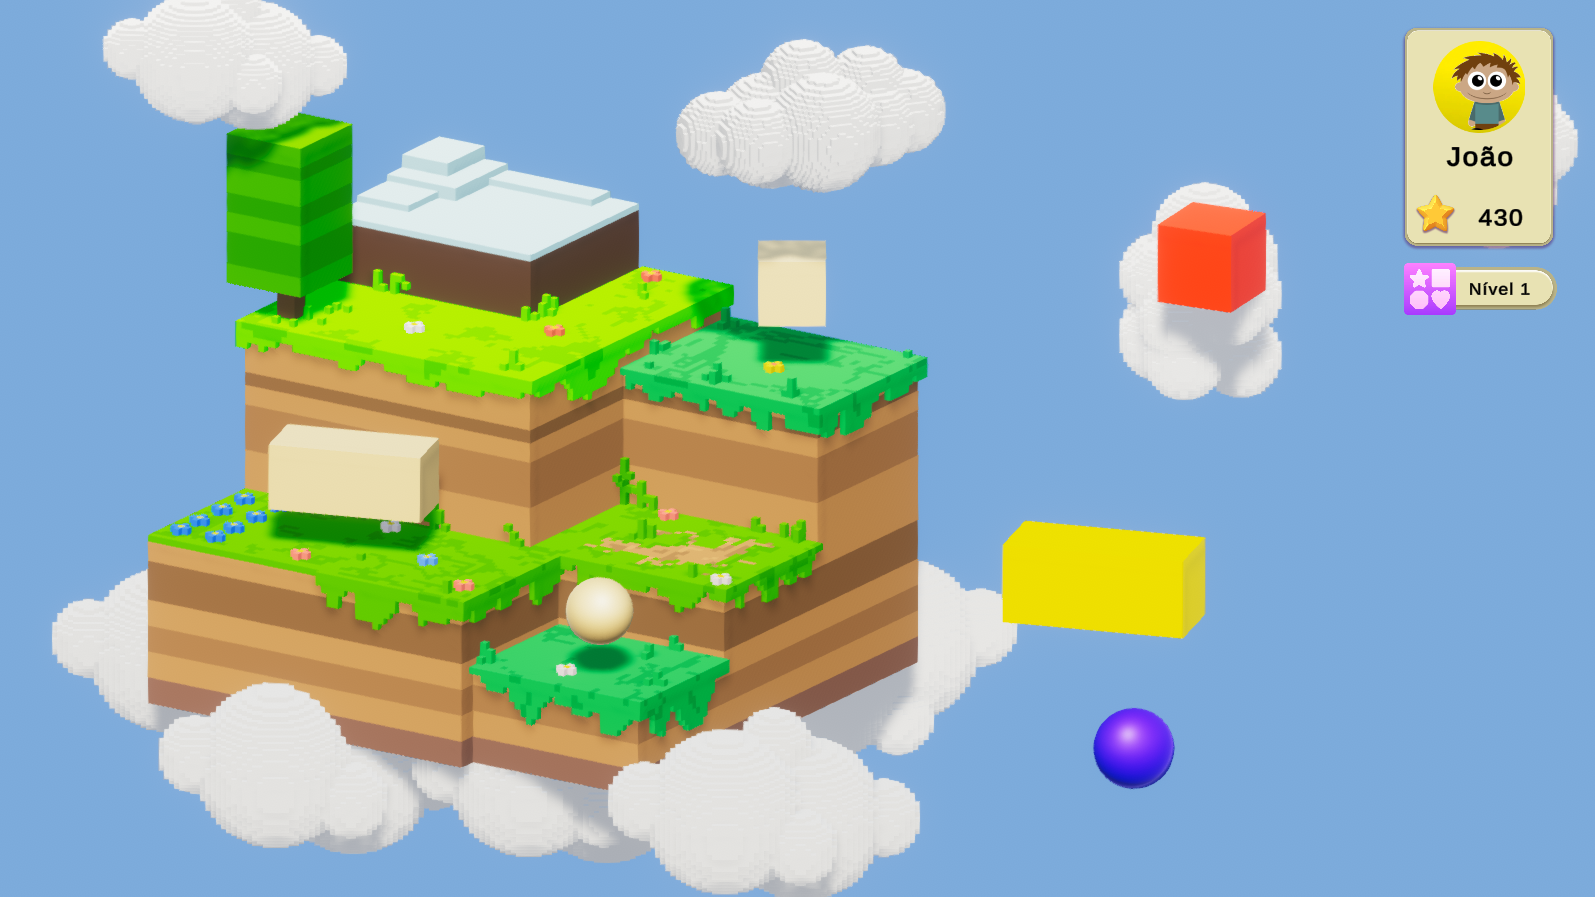
\includegraphics[width=0.8\linewidth]{GameScreenshots/Level1.png}
\end{figure}

\normalfont
\begin{tasks}[style=enumerate, item-format={\normalfont\tiny}, after-item-skip=4mm](6)
\task Não atende
\task 
\task 
\task 
\task Atende completamente
\end{tasks}

\textbf{Pergunta 7} - "Utilizar sons produzidos por materiais, objetos e instrumentos musicais durante brincadeiras ...", entre 1 e 5 o quanto você considera que o nível 2 do jogo atende esta finalidade?

\begin{figure}[H]
    \centering
    \label{fig:aluno_pergunta_5}
    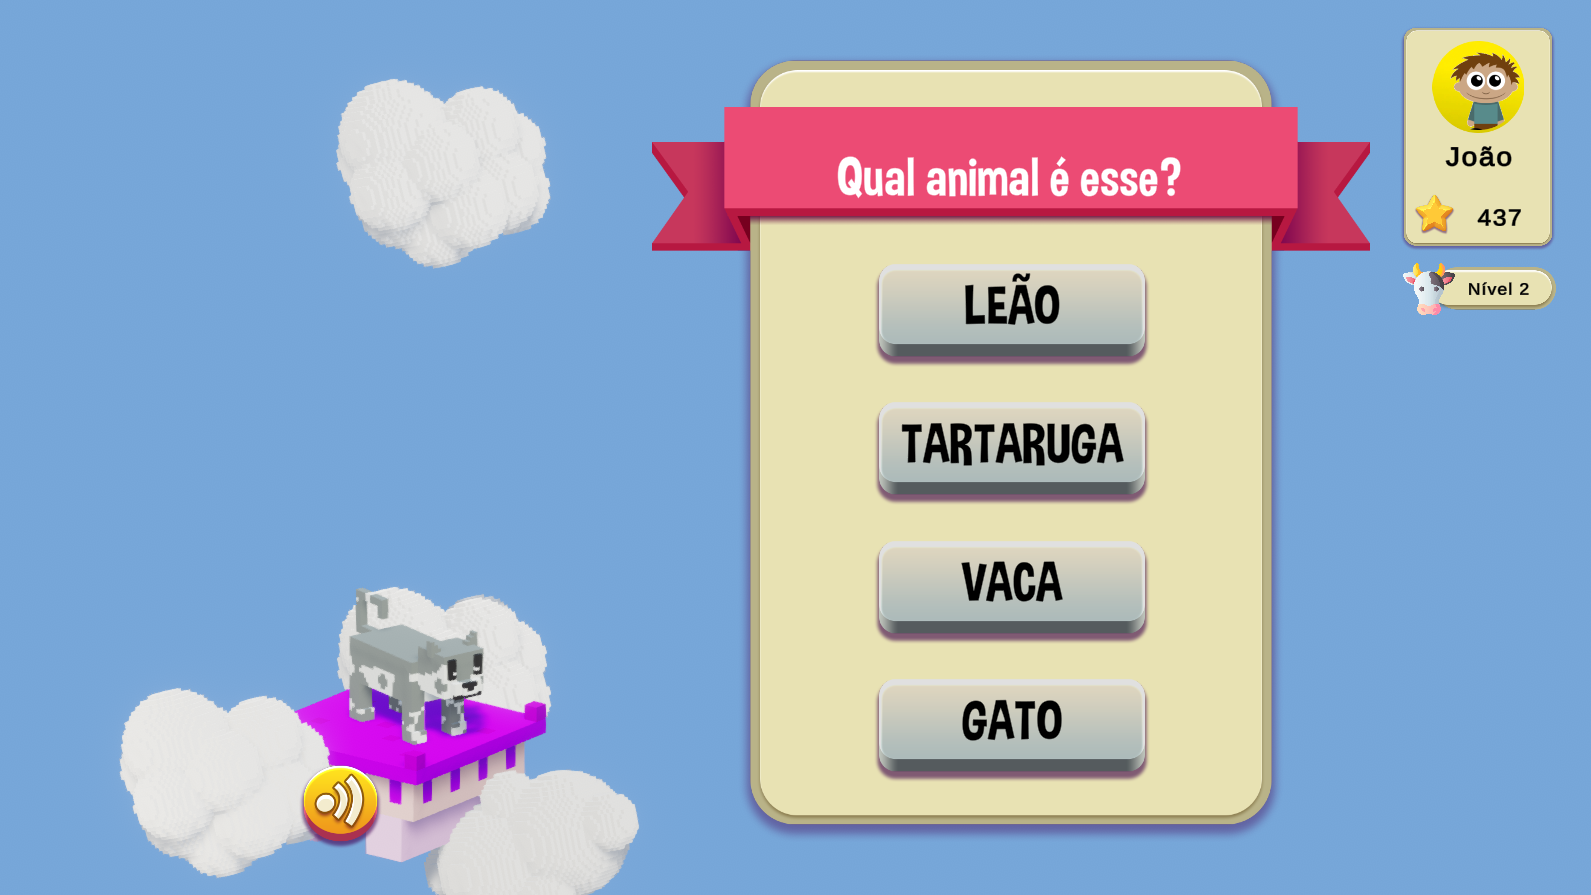
\includegraphics[width=0.8\linewidth]{GameScreenshots/Level2.png}
\end{figure}

\normalfont
\begin{tasks}[style=enumerate, item-format={\normalfont\tiny}, after-item-skip=4mm](6)
\task Não atende
\task 
\task 
\task 
\task Atende completamente
\end{tasks}

\textbf{Pergunta 8} - "Classificar objetos e figuras de acordo com suas semelhanças e diferenças", entre 1 e 5 o quanto você considera que o nível 3 do jogo atende esta finalidade?

\begin{figure}[H]
    \centering
    \label{fig:aluno_pergunta_5}
    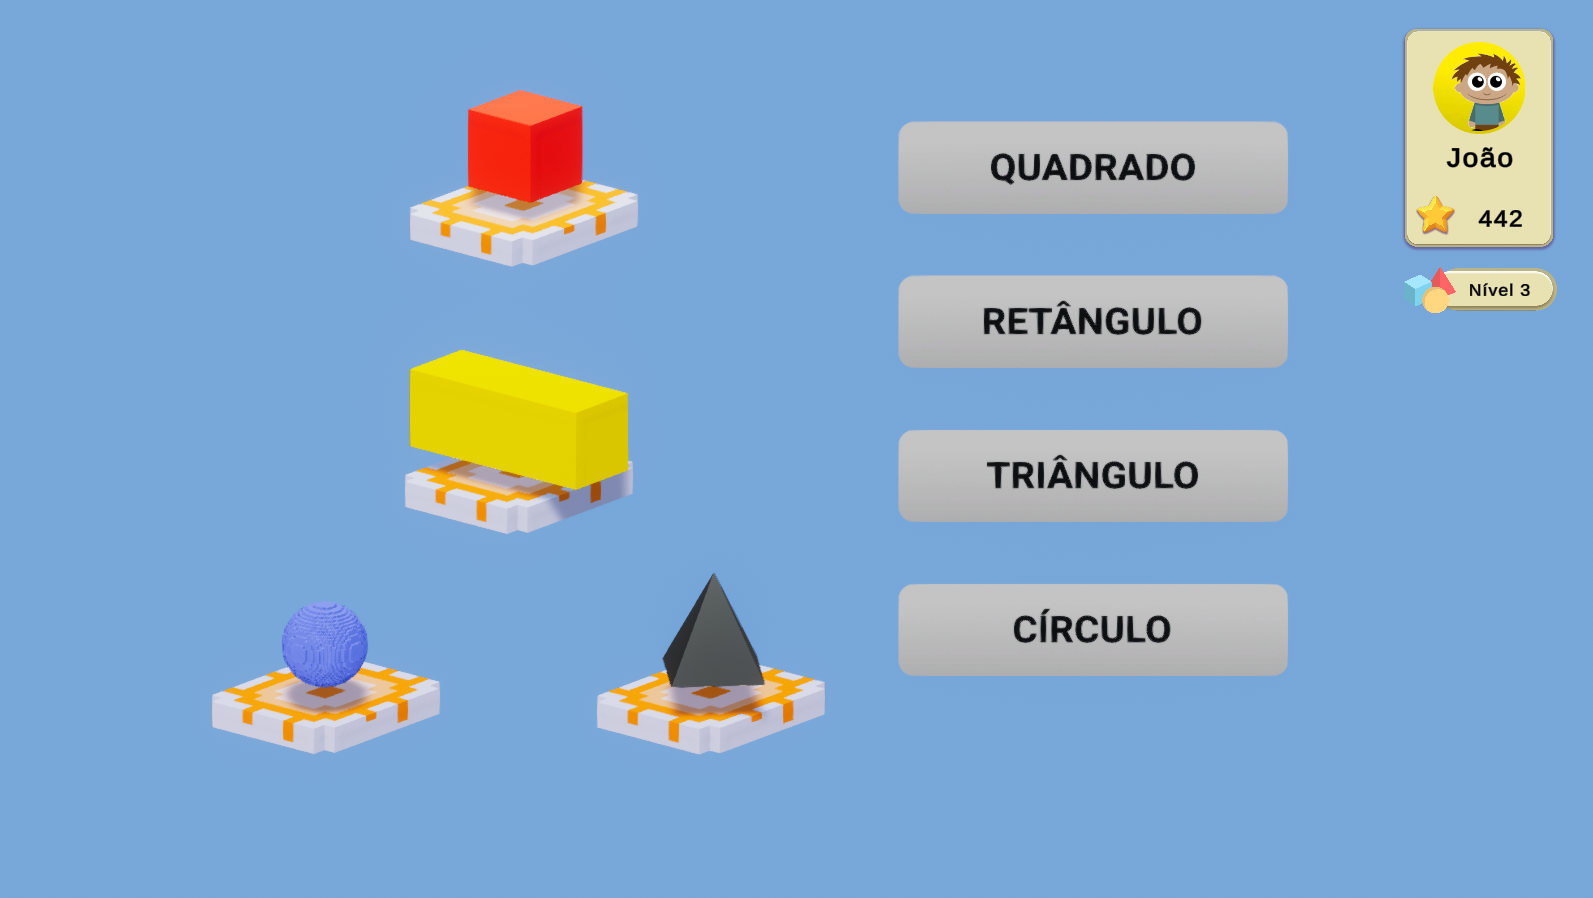
\includegraphics[width=0.8\linewidth]{GameScreenshots/Level3.png}
\end{figure}

\normalfont
\begin{tasks}[style=enumerate, item-format={\normalfont\tiny}, after-item-skip=4mm](6)
\task Não atende
\task 
\task 
\task 
\task Atende completamente
\end{tasks}

\textbf{Pergunta 9} - "Estabelecer relações de comparação entre objetos, observando suas propriedades.", entre 1 e 5 o quanto você considera que o nível 4 do jogo atende esta finalidade?

\begin{figure}[H]
    \centering
    \label{fig:aluno_pergunta_5}
    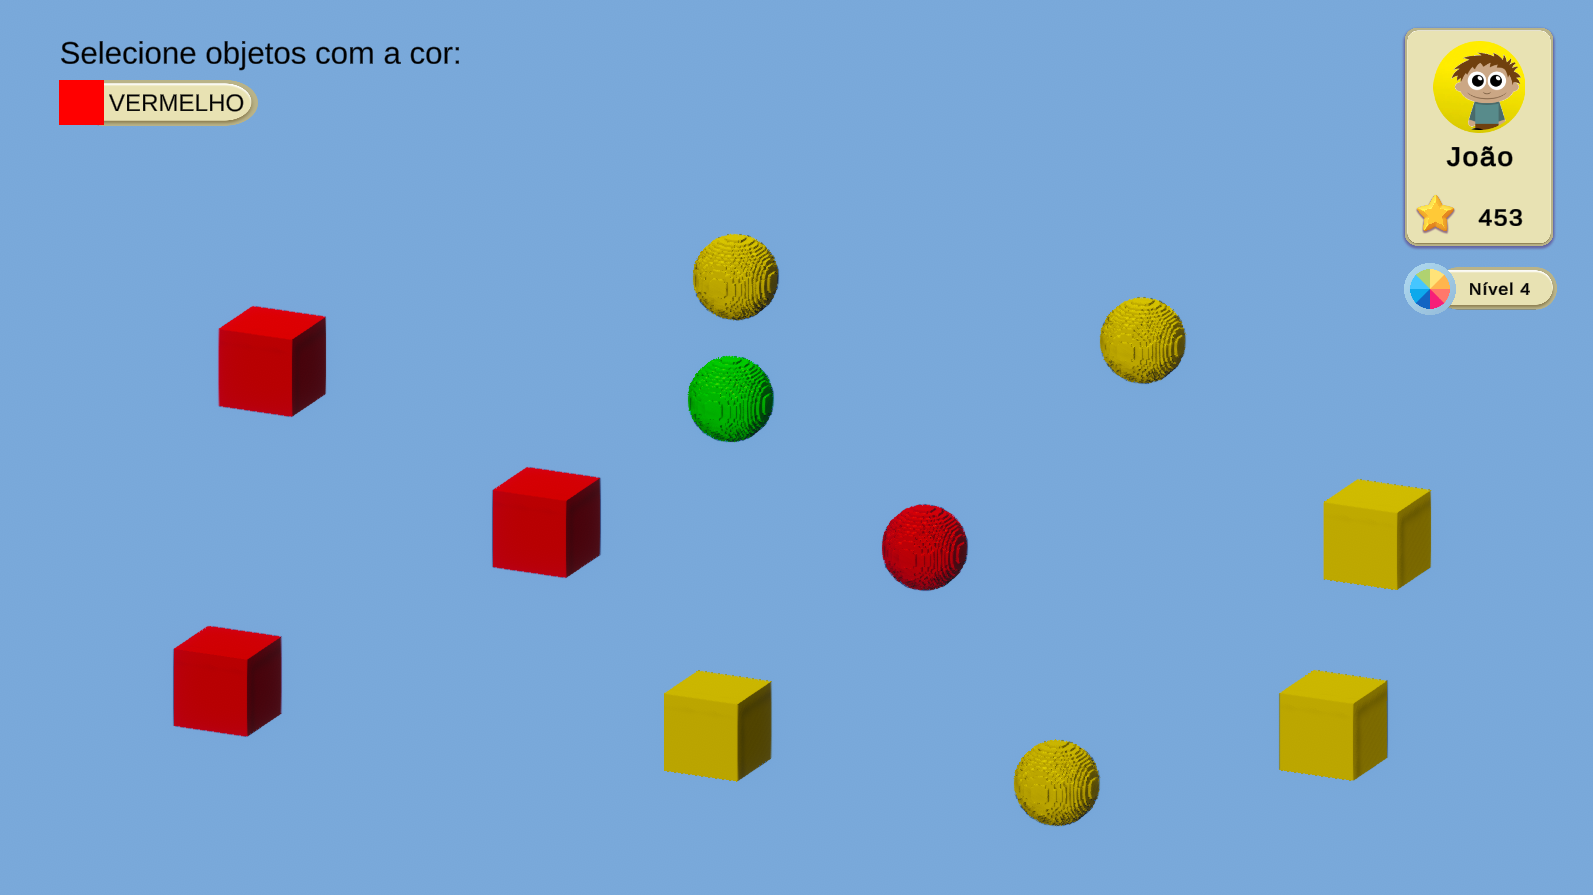
\includegraphics[width=0.8\linewidth]{GameScreenshots/Level4.png}
\end{figure}

\normalfont
\begin{tasks}[style=enumerate, item-format={\normalfont\tiny}, after-item-skip=4mm](6)
\task Não atende
\task 
\task 
\task 
\task Atende completamente
\end{tasks}

\textbf{Pergunta 10} - Você utilizaria de um jogo virtual educativo em sala como ferramenta complementar à sua aula?
\begin{itemize}
     \item Sim
     \item Não
\end{itemize}

\textbf{Pergunta 11} - Se não, justifique sua resposta:

\textbf{Pergunta 12} - Você considera que teria aptidão para utilizar de recursos tecnológicos, tais como: computador, mouse e teclado?
\begin{itemize}
     \item Sim, muita aptidão
     \item Sim, pouca aptidão
     \item Não, nenhuma aptidão
\end{itemize}

\textbf{Pergunta 13} - Você julga necessário um treinamento para a utilização desses recursos?
\begin{itemize}
     \item Sim
     \item Não
\end{itemize}

\textbf{Pergunta 14} - Se sim, como esse treinamento deveria ocorrer?
\begin{todolist}
     \item Online
     \item Na sua instituição
     \item Em outra instituição
     \item Por meio de apostilas e materiais diversos
     \item Outro...
\end{todolist}

\textbf{Pergunta 15} - Deseja fazer algum comentário, observação e/ou crítica? Escreva para gente:

\end{document}
